\documentclass[fleqn]{beamer}
\usepackage{pgfpages}

\setbeamertemplate{note page}[plain]
\setbeameroption{show notes on second screen=bottom}
\usetheme{Madrid}
\beamertemplatenavigationsymbolsempty

\usepackage[utf8]{inputenc}
% font - Palatino
\usepackage[sc,osf]{mathpazo}   % With old-style figures and real smallcaps.
\usepackage[euler-digits,small]{eulervm}
\usepackage[style=authortitle-comp, backend=biber]{biblatex}
\usepackage{xpatch}
\xapptobibmacro{cite}{\setunit{\nametitledelim}\printfield{year}}{}{}
\addbibresource{./references.bib}
\usepackage[compat=1.1.0]{tikz-feynman}
\usepackage{bm}
\usepackage{commath}
\usepackage{booktabs} % \toprule, \midrule
\usepackage{multirow} % \multirow
\usepackage{tabularx}
\usepackage{colortbl} % \rowcolor in tables
\usepackage{adjustbox} % \resizebox for table
\usepackage{xcolor}
\usepackage{caption}
\usepackage{siunitx}
\usepackage{appendixnumberbeamer}
\usepackage{booktabs} % \toprule etc.
\usepackage{nccmath} % center equation
\usepackage{tikz}
\usetikzlibrary{positioning}
\usetikzlibrary{arrows}


\DeclareMathOperator{\Ima}{Im}
\DeclareMathOperator{\sfm2}{sfm2}
\DeclareMathOperator{\cov}{cov}

\definecolor{primary}{rgb}{0.78, 0.89, 1}
\setbeamercolor{palette primary}{fg=white,bg=black!80}
\setbeamercolor{palette secondary}{fg=white,bg=black!40}
\setbeamercolor{palette tertiary}{fg=black,bg=black!20}
\setbeamercolor{caption name}{fg=black}
\setbeamercolor{block title}{bg=black!40}

\setbeamertemplate{section in toc}{ {\color{black}\inserttocsectionnumber.~\inserttocsection} }
\setbeamertemplate{subsection in toc}{ \hspace{1.2em}{\color{black}\rule[0.3ex]{3pt}{3pt}}~\inserttocsubsection\par }
\setbeamertemplate{itemize items}[square]

\setbeamertemplate{blocks}[default]
\setbeamerfont{caption}{size=\tiny}

\setbeamerfont{myTOC}{size=\normalsize}
\AtBeginSection[]{
  \ifnum \value{framenumber}>1
    \frame{\frametitle{Outline}\usebeamerfont{myTOC}\tableofcontents[current,subsubsectionstyle=hide]}
  \else
  \fi
}

\makeatletter
\setbeamertemplate{footline}
{
  \leavevmode%
  \hbox{%
    \begin{beamercolorbox}[wd=.333333\paperwidth,ht=2.25ex,dp=1ex,center]{author in head/foot}%
      \usebeamerfont{author in head/foot}\insertsection
    \end{beamercolorbox}%
    \begin{beamercolorbox}[wd=.333333\paperwidth,ht=2.25ex,dp=1ex,center]{title in head/foot}%
      \usebeamerfont{title in head/foot}\insertsubsection
    \end{beamercolorbox}%
    \begin{beamercolorbox}[wd=.333333\paperwidth,ht=2.25ex,dp=1ex,right]{date in head/foot}%
      \usebeamerfont{date in head/foot}\insertshortdate{}\hspace*{2em}
      \insertframenumber{} / \inserttotalframenumber\hspace*{2ex} 
    \end{beamercolorbox}}%
  \vskip0pt%
}
\makeatother


\title[The Strong Coupling]{The QCD Strong Coupling from Hadronic Tau Decays}
\subtitle{A PhD Defense}
\author{Dirk Hornung}
\institute[UAB]{
  Universitat Autònoma de Barcelona \\
  \tiny
  Departamiento de Física
}
\titlegraphic{
  
\includegraphics[height=1.5cm]{./images/logo_UAB.eps}
  \hspace{1cm}
  
\includegraphics[height=1.5cm]{./images/logo_IFAE.eps}
}
\date{17th July 2019}

\begin{document}
\frame{\titlepage}

\section{Introduction}
\begin{frame}
  \frametitle{The Strong Coupling \(\alpha_s\)}
  \begin{equation} 
    \begin{split}
      \mathcal{L}_{QCD}(x) &= -\frac{1}{4} G_{\mu\nu}^a(x) G^{\mu\nu,a}(x) \\
      &+ \left[ \sum_A \frac{i}{2} \overline{q}^A(x) \gamma^\mu \overleftrightarrow{D}_\mu q^A(x) - m \overline{q}^A(x)q^A(x) \right],
    \end{split}
  \end{equation}
  \small
  with \(D_\mu = \partial_\mu - i g \frac{\lambda^a}{2} B_\mu^a\)
  \note{say hello now}

  \pause
  \normalsize
  \begin{equation}
    \mathcal{L}_{QCD}^{QG-Int}(x) = \sqrt{\pi \bm{\alpha_s}} \, \overline{q}(x) \lambda \gamma_\mu q (x) G(x)
    \quad \Rightarrow \quad
    \feynmandiagram [inline=(d.base), horizontal=d to b] {
      a [particle=\(\overline{q}\)] -- [fermion] b -- [fermion] c [particle=\(q\)],
      b -- [boson, edge label=\(g\)] d,
    };
  \end{equation}
\end{frame}
\begin{frame}
  \frametitle{The Running of the Strong Coupling}
  \begin{columns}
    \begin{column}{0.4\textwidth}
      \begin{equation}
        \begin{split}
          \alpha_s(m_\tau^2) &\approx 0.33 \\
          \alpha_s(m_Z^2) &\approx  1.12
        \end{split}
      \end{equation}
        \begin{equation}
          \footnotesize
          \begin{split}
            m_\tau &= \SI{1776.86 \pm 0.12}{\mega\eV}\footnotemark \\
            m_Z &= \SI{91.1876 \pm 0.0021}{\giga\eV}^1
          \end{split}
        \end{equation}
    \end{column}
    \begin{column}{0.5\textwidth}
      \begin{figure}
        \includegraphics[width=\textwidth]{./images/runningOfAs.eps}\\[-1ex]
        \captionsetup{format=hang}
        \caption{\tiny Taken from \cite{Deur2016}}
      \end{figure}
    \end{column}
  \end{columns}
  \footnotetext{\cite{PDG2018}}
\end{frame}
\begin{frame}
  \frametitle{Hadronic \(\tau\) decays}
  \begin{columns}
    \begin{column}{0.4\textwidth}
      \feynmandiagram [layered layout, horizontal=a to b] {
        a [particle=\(\tau^{-}\)] -- [fermion] b -- [fermion] f1 [particle=\(\nu_{\tau}\)], b -- [boson, edge label'=\(W^{-}\)] c,
        c -- [anti fermion] f2 [particle=\(\overline{u}\)],
        c -- [fermion] f3 [particle=\(d\)],
      };
    \end{column}

    \pause
    \begin{column}{0.6\textwidth}
      \begin{equation}
        R_\tau = \frac{\Gamma[\tau^- \to \nu_\tau + \text{hadrons}]}{\Gamma[\tau^- \to \nu_\tau e^- \overline{\nu}_{e}]}
      \end{equation}
    \end{column}
  \end{columns}

  \vspace{1cm}
  
  \pause
  \centering
  \begin{tabular}{lccc}
    \toprule
    Name & Symbol & Quark content & Rest mass \\
    \midrule
    Pion & \(\pi^-\) & \(\overline{u} d\) & \SI{139.57061 \pm 0.00024}{\mega\eV}  \\
    Pion & \(\pi^0\) & \((u \overline{u} - d \overline{d})/\sqrt{2}\) & \SI{134.9770\pm0.0005}{\mega\eV}
  \end{tabular}
\end{frame}
\begin{frame}
  \frametitle{Duality}
  \centering
  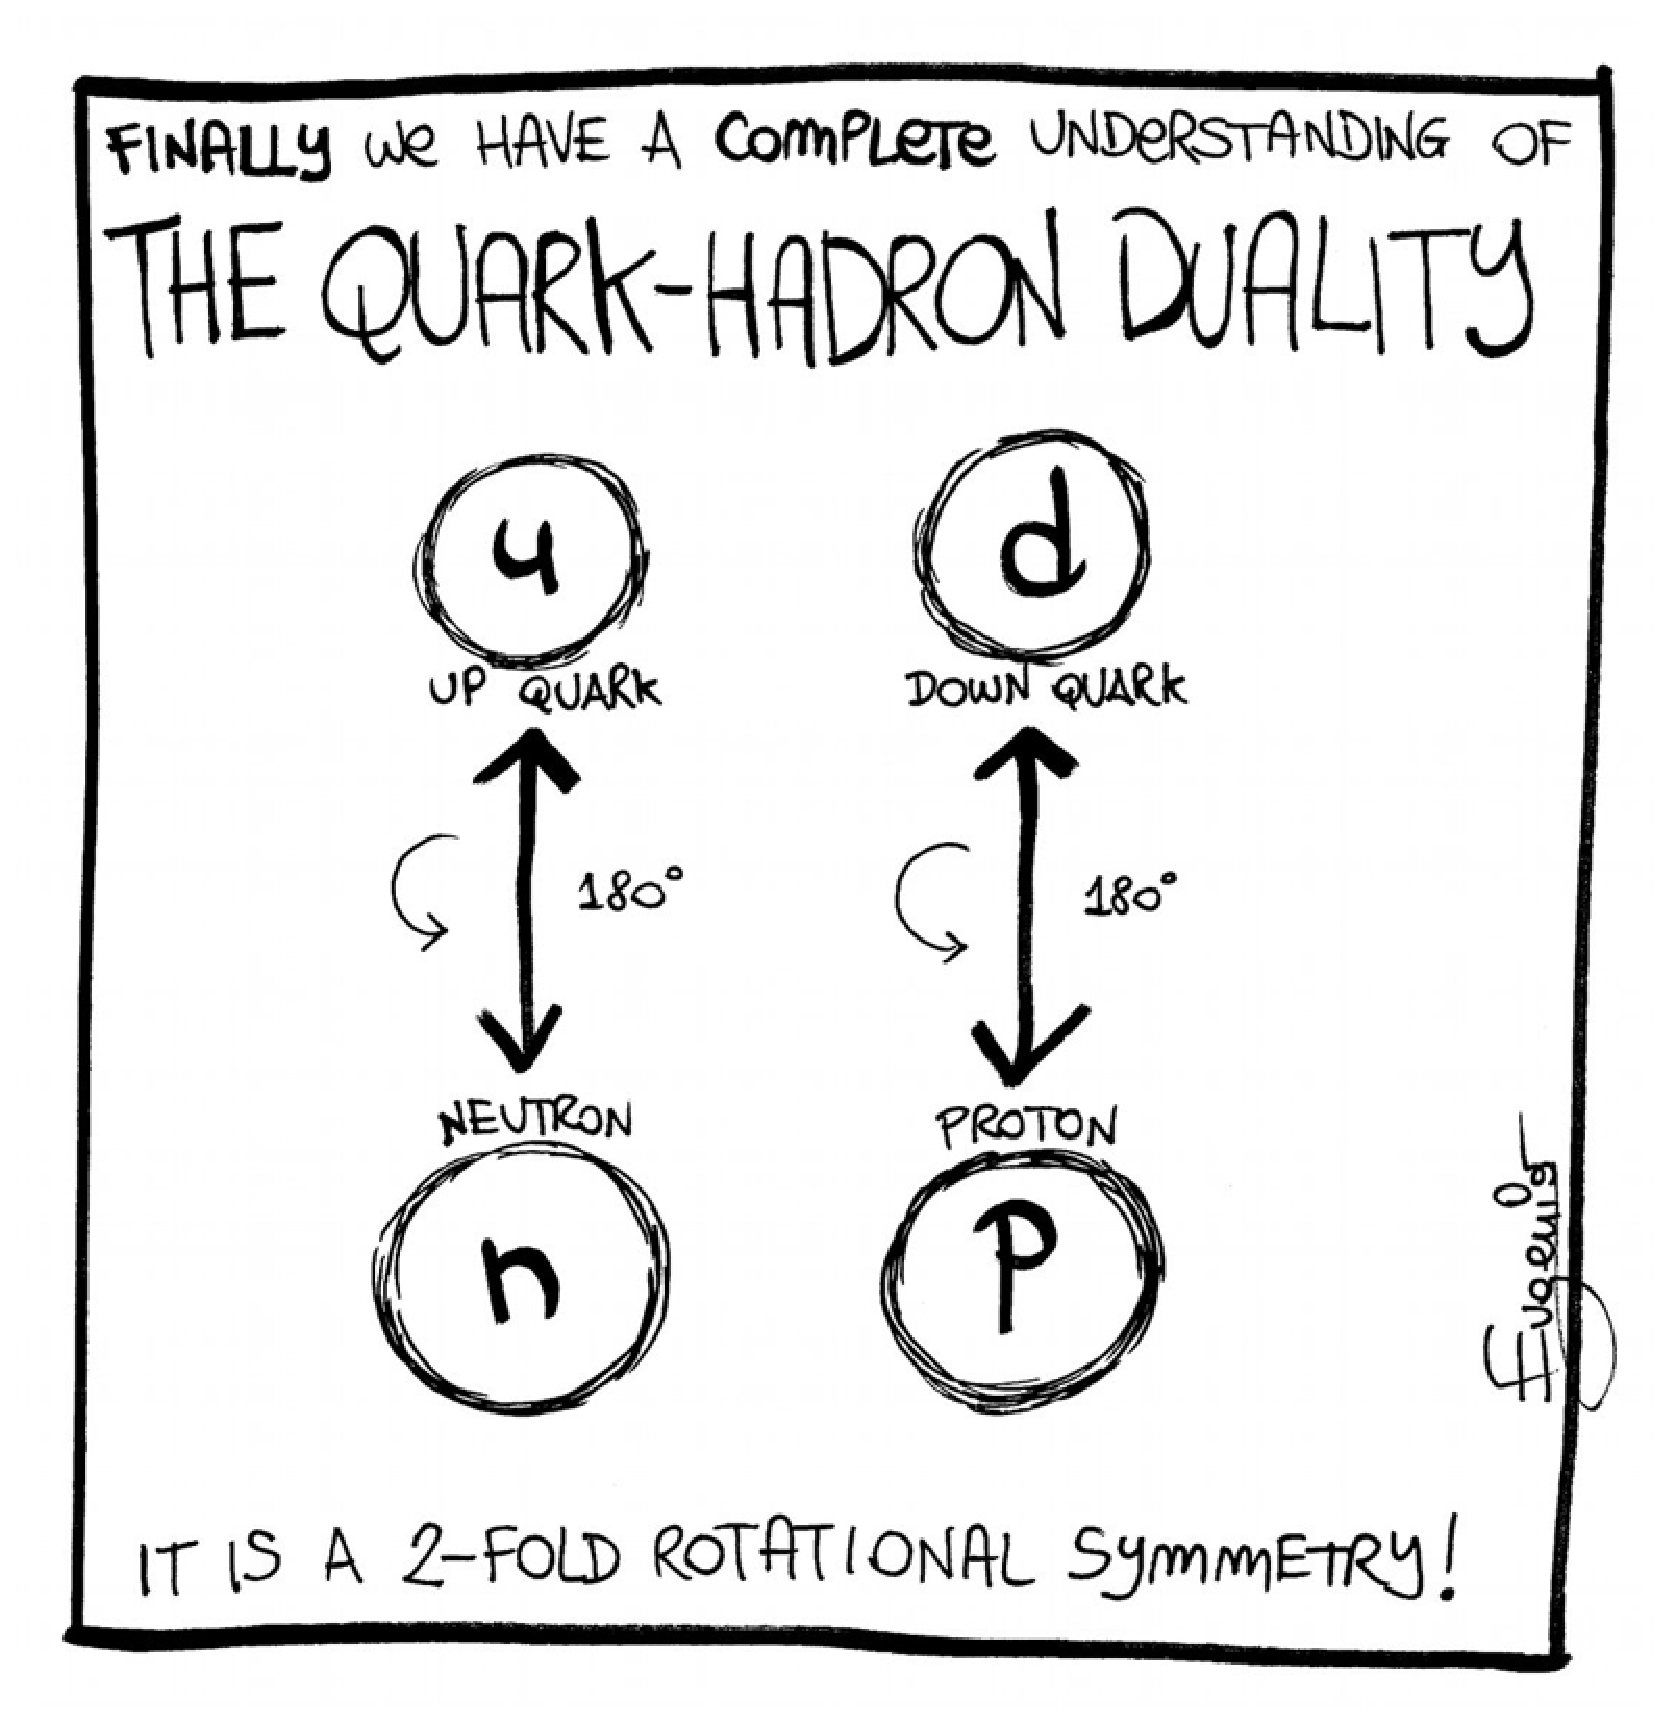
\includegraphics[width=0.5\textwidth]{./images/quarkHadronDuality.eps}
\end{frame}

\begin{frame}
  \frametitle{Table of Contents}
  \tableofcontents[subsubsectionstyle=hide]
\end{frame} 

\section{Theoretical Framework}
\subsection{Two-Point Function}
\begin{frame}
  \frametitle{Two-Point Function}
  \begin{block}{Two-Point Function:}
    \begin{ceqn}
      \begin{equation}
        \begin{split}
          \Pi_{V/A}^{\mu\nu}(q^2) &\equiv i \int \dif^4 x e^{iqx} \langle 0\vert T \left\{ J_{V/A}^\mu(x) J_{V/A}^\nu(0)\right\} \vert 0 \rangle \\
          &= (q^\mu q^\nu - q^2 g^{\mu\nu})\Pi_{V/A}^{(1)}(q^2) + q^\mu q^\nu \Pi_{V/A}^{(0)}(q^2) \\
          &= (q^\mu q^\nu - q^2 g^{\mu\nu}) \Pi^{(1+0)}_{V/A}(q^2) + q^2 g_{\mu\nu} \Pi^{(0)}(q^2) 
        \end{split}
      \end{equation}
    \end{ceqn}
  \end{block}

  \vspace{0.5cm}

  \small\centering
  \(J_V^\mu = \overline{u} \gamma^\mu d \qquad \text{and} \qquad J_A^\mu = \overline{u} \gamma^\mu \gamma_5 d\)
\end{frame}
\note[itemize] {
  \item Two-point function 
  \item \(J_{V/A}^{\mu}\) is the non-strange \(V\) or \(A\) current
  \item superscripts \((0)\) and \((1)\) label spin
  \item Lorentz decomposed
  \item \(\Pi^{(1+0)}(q^2) q^2 \Pi^{(0)}(q^2)\) free of kinematic singularities
}

\subsection{QCD Sum Rules}
\begin{frame}
  \frametitle{Cauchy's Theorem}
  
  \centering
  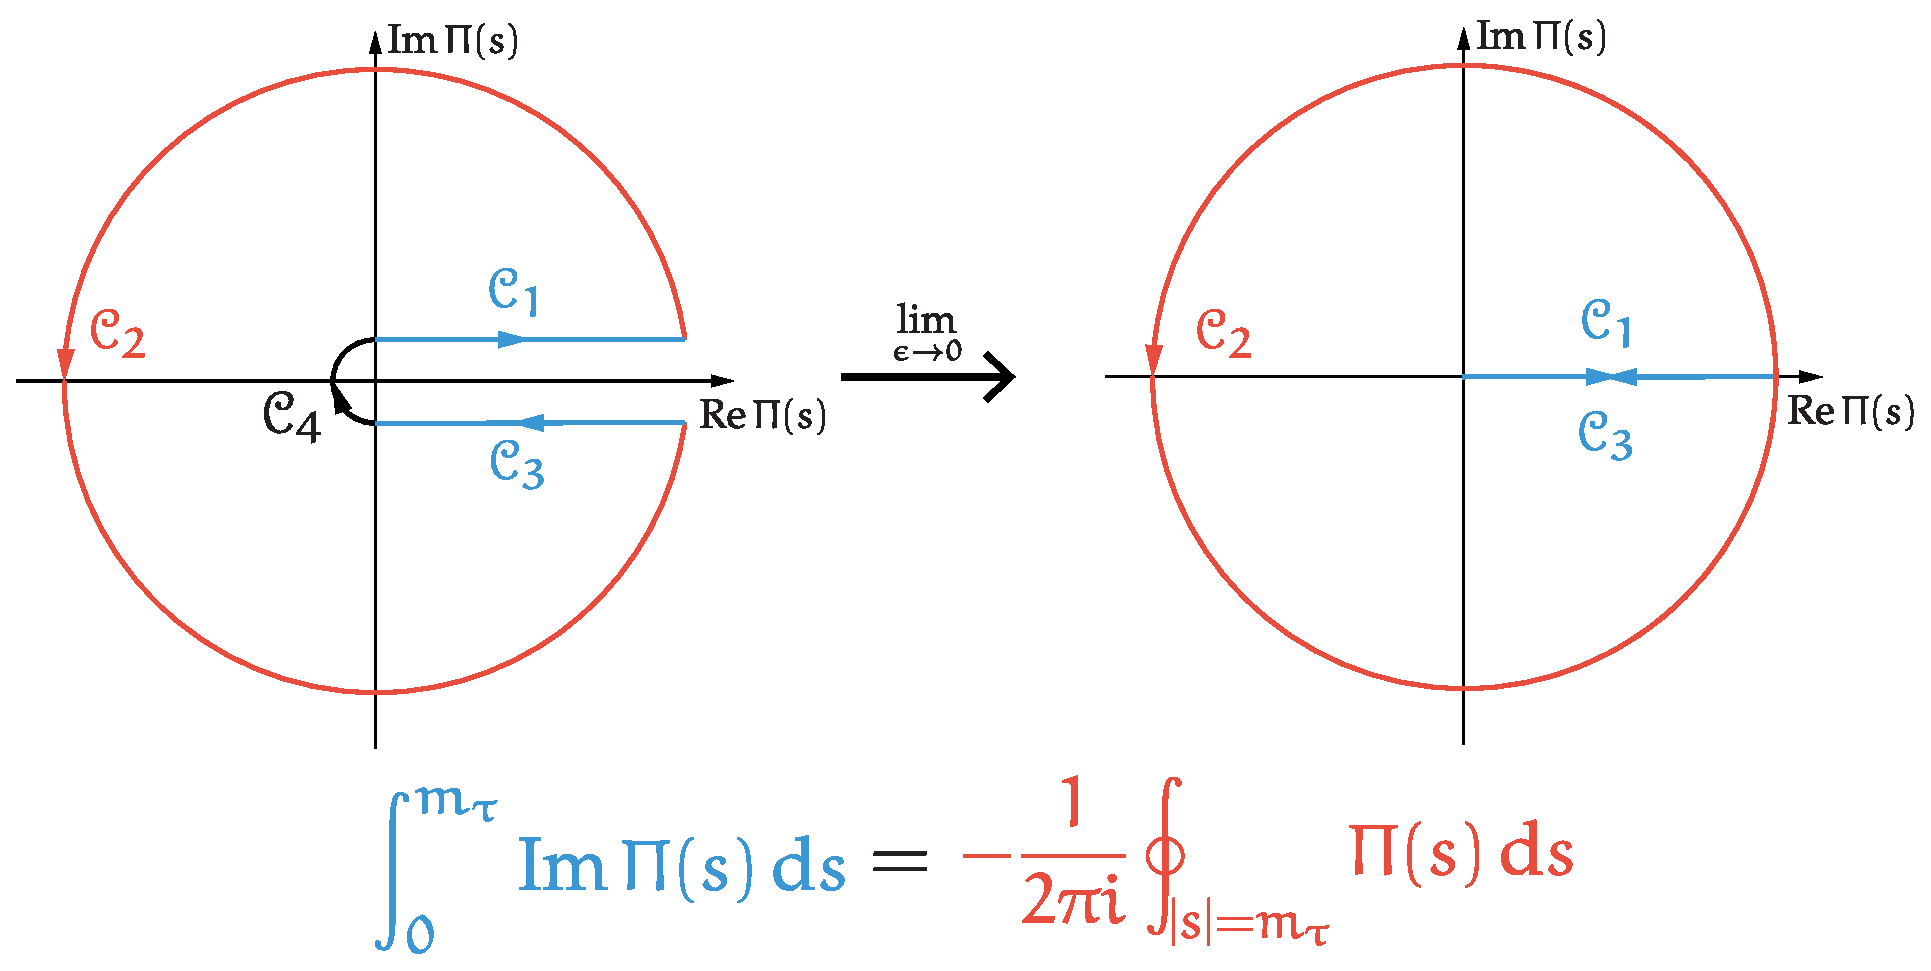
\includegraphics[width=0.8\textwidth]{./images/rTauCauchysTheorem.eps}

  \vspace*{0.5cm}

\end{frame}
\note[itemize]{
  \item Experimental data only accessible on positive real axis
  \item Imaginary part of two-point function related to experimental accessible
    spectral function
  \item integrate from \(0\) to \(m_\tau^2\) to reproduce \(R_\tau(m_\tau^2)\)
  \item Theoretically the positive real axis is not accessible
  \item Two-point function has poles on positive real axis
  \item \(\Rightarrow \quad\) Cauchy's theorem
  \item Identify 
}

\begin{frame}
  \frametitle{Finite Energy Sum Rule (FESR)}
  Spectral Function
  \begin{ceqn}
    \begin{equation}
      \rho^{(1+0)}(s) = \frac{1}{\pi} \Ima \Pi^{(1+0)}(s)
    \end{equation}
  \end{ceqn}

  \vfill

  % \begin{block}{\vspace*{-3ex}}
  \begin{block}{Spectral Moment}
    \begin{ceqn}
      \begin{equation}
        I_{V/A}^{\omega}(s_0) \equiv \frac{1}{s_0} \int_{0}^{s_0} \dif s \, \omega\left(\frac{s}{s_0}\right) \rho(s) = \frac{-1}{2 \pi i s_0} \oint_{\abs{s}=s_0} \dif s \, \omega\left(\frac{s}{s_0} \right) \Pi(s)
      \end{equation}
    \end{ceqn}
  \end{block}
\end{frame}
\note[itemize]{
  \item Spectral function equal to the imaginary part of the correlator
  \item Spectral function is given by the experiment
  \item Experiment only valid to certain energy \(s_0\)
  \item \(\Rightarrow\) \textit{Finite Energy} Sum Rule
  \item Define spectral moment
  \item Introduce weights
  \item Weights \(\omega\) have to be analytic
}

\begin{frame}
  \frametitle{Adler Function}
  Adler Function:
  \begin{equation}
    D(s) \equiv s \frac{\dif}{\dif s} \Pi(s)
  \end{equation}
  \begin{equation}
    \begin{split}
      R_{\tau, V/A}^{\omega}(s_0) &\equiv \frac{12 \pi^2}{s_0} \int_{0}^{s_0} \dif s \, \omega\left( \frac{s}{s_0} \right) \rho(s) \\
      &= \frac{6 \pi i}{s_0} \oint_{\abs{s}=s_0} \dif s \, \omega\left(\frac{s}{s_0} \right) \Pi(s) \\
      &= -3 \pi i \oint_{\abs{x}=1} \frac{\dif x}{x} \omega_D(x) D(x s_0),
    \end{split}
  \end{equation}
  where \(x \equiv \frac{s}{s_0}\)and \(\omega_D \equiv 2 \int_x^1
  \dif \omega{x}\)
  % \begin{equation}
  %   D^{(1+0)}(s) \equiv -s \frac{\dif}{\dif s} \Pi^{(1+0)}(s), \qquad D^{(0)}(s) \equiv \frac{s}{m_\tau^2} \frac{\dif}{\dif s} \left( s \Pi^{(0)}(s) \right)
  % \end{equation}
\end{frame}
\note[itemize]{
  \item Adler Function for convenience
  \item In case of vector correlator the derivative (Adler Function) is a
    physical quantity
  \item Physical quantities are renormalisation scale invariant
  \item For the \((1+0)\) and \((0)\) we use a different definition
}

\subsection{Operator Product Expansion}
\begin{frame}
  \frametitle{Operator Product Expansion}
  \begin{equation}
    \Pi_{OPE}(q^2) = -\frac{1}{3 q^2}\sum_n \langle\Omega\vert \mathcal{O}_n(0) \vert\Omega\rangle \int \dif^4\, e^{iqx} C_n(x)
  \end{equation}
  \begin{equation}
    \begin{split}
    \Pi_{OPE, V/A}(s) &= \sum_{D=0,2,4,\dots} \frac{C^{(D)} \langle\Omega\vert \mathcal{O}^{(D)}(x) \vert\Omega\rangle}{(s)^{D/2}} \\
    &= \underbrace{\vphantom{\sum_{k=1}^\infty} C_0}_{PT} + \underbrace{\sum_{k=1}^\infty \frac{C_{2k}(s)}{s^k}}_{NPT}
  \end{split}
\end{equation}
\end{frame}


\subsection{Perturbative Contributions}
\begin{frame}
  \frametitle{Perturbative Contributions}
  \begin{equation}
    \Pi_V^{(1+0)}(s) = - \frac{N_c}{12 \pi^2} \sum_{n=0}^\infty a_\mu^n \sum_{k=0}^{n+1} c_{n,k} L^k
    \quad \text{with} \quad L \equiv \log \frac{-s}{\mu^2}
  \end{equation}

  \begin{equation}
    D_V^{(1+0)} = \frac{N_c}{12 \pi^2} \sum_{n=0}^\infty a_\mu^n \sum_{k=1}^{n+1} k\, c_{n,k} L^{k-1}
  \end{equation}

\end{frame}

\begin{frame}
  \frametitle{Adler Function Coefficients}
  \centering
  \begin{block}{Renormalisation Group Equation}
    \begin{ceqn}
      \begin{equation}
        \mu \frac{\dif}{\dif \mu} R(q, a_s, m) = \left[ \mu \frac{\partial}{\partial \mu} + \mu \frac{\dif a_s}{\dif \mu} \frac{\partial}{\partial a_s} + \mu \frac{\dif m}{\dif \mu} \frac{\partial}{\partial m} \right] R(q, a_s, m) = 0
      \end{equation}
    \end{ceqn}
  \end{block}
  \begin{ceqn}
    \begin{equation}
      \left(2 \frac{\partial}{\partial L} + \beta \frac{\partial}{\partial a_s} \right) D_V^{(1+0)} = 0
    \end{equation}
  \end{ceqn}
  \begin{columns}
    \begin{column}{.5\textwidth}
      \begin{scriptsize}
        \begin{equation}
          \begin{split}
            c_{0,0} &= -\frac{5}{3}, \quad c_{0,1} = 1, \\
            c_{1,1} &= 1 \\
            c_{2,1} &= \frac{365}{24} - 11 \zeta_3 - ( \frac{11}{12} - \frac{2}{3}\zeta_3 ) N_f \\
            \cdots
          \end{split}
        \end{equation}
      \end{scriptsize}
    \end{column}
    \begin{column}{.5\textwidth}
      \begin{scriptsize}
        \begin{equation}
          \begin{split}
            c_{2,2} &= -\frac{1}{4} \beta_1 c_{1,1}, \\
            c_{3,2} &= \frac{1}{4}(-\beta_2 c_{1,1} - 2 \beta_1 c_{2,1}), \\
            c_{3,3} &= \frac{1}{12}\beta_1 c_{1,1} \\
            \cdots
          \end{split}
        \end{equation}
      \end{scriptsize}
    \end{column}
  \end{columns}
\end{frame}
\note[itemize]{
  \item Beta function definition missing
}

\begin{frame}
  \frametitle{Perturbative Contribution}
  \begin{small}
    \begin{equation}
      \delta_{pt} = \sum_{n=1}^\infty a_\mu^n \sum_{k=1}^n k\, c_{n,k} \frac{1}{2 \pi i} \oint_{\abs{x}=1} \frac{\dif x}{x} (1-x)^3 (1+x) \log \left( \frac{-m_\tau^2 x}{\mu^2} \right)^{k-1}
    \end{equation}
    \centering
    \begin{tikzpicture}[>=triangle 45,font=\sffamily]
      \node (X) at (0,0) {};
      \node (Y) [below left=1.5cm and 3cm of X]  {};% 2cm below, 1cm to the left (optional)
      \node (Z) [below right=1.5cm and 3cm of X] {};
      \draw [semithick,->] (X) -- (Y);
      \draw [semithick,->] (X) -- (Z);
    \end{tikzpicture}
    \begin{columns}
      \begin{column}{.5\textwidth}
        \centering
        Fixed-Order Perturbation Theory (FOPT)
        \begin{ceqn}
          \begin{equation*}
            \mu \equiv m_\tau^2
          \end{equation*}
        \end{ceqn}
      \end{column}
      \begin{column}{.5\textwidth}
        \centering
        Contour-Improved Perturbation Theory (CIPT)
        \begin{ceqn}
          \begin{equation}
            \mu \equiv -m_\tau^2 x
          \end{equation}
        \end{ceqn}
      \end{column}
    \end{columns}
  \end{small}
\end{frame} 

\begin{frame}
  \frametitle{Fixed-Order Perturbation Theory}
  \begin{equation}
    \delta_{FOPT}^{(0)} = \sum_{n=1}^\infty a(m_\tau^2)^n \sum_{k=1}^n k\, c_{n,k} J_{k-1}
  \end{equation}
  \begin{equation}
    J_l \equiv \frac{1}{2\pi i} \oint_{\abs{x}=1} \frac{\dif x}{x} (1-x)^3 (1+x) \log^l(-x)
  \end{equation}
\end{frame}
\begin{frame}
  \frametitle{CIPT}
  \begin{equation}
    \delta_{CIPT}^{(0)} = \sum_{n=1}^\infty c_{n,1}\, J_n^a(m_\tau^2)
  \end{equation}
  \begin{equation}
    J_n^a(m_\tau^2) \equiv \frac{1}{2 \pi i} \oint_{\abs{x}=1} \frac{\dif x}{x} (1-x)^3 (1+x) a^n (-m_\tau^2 x)
  \end{equation}
\end{frame}

\begin{frame}
  \frametitle{FOPT vs CIPT}
  \begin{footnotesize}
    \begin{align}
      & \quad\qquad \alpha_s^2 \qquad \alpha_s^2 \qquad \alpha_s^3 \qquad \alpha_s^4 \quad\qquad \alpha_s^5 \nonumber\\
      \delta_{FOPT}^{(0)} &= 0.1082 + 0.0609 + 0.0334 + 0.0174 (+ 0.0088) = 0.2200 (0.2288) \\
      \delta_{CIPT}^{(0)} &= 0.1479 + 0.0297 + 0.0122 + 0.0086 (+ 0.0038) = 0.1984 (0.2021)
    \end{align}
  \end{footnotesize}
\end{frame}

\begin{frame}
  \frametitle{Borel Summation}
  Borel integral
  \begin{equation}
    A \equiv \int_0^\infty \dif t e^{-t} \sum_{n=0}^\infty \frac{a_k}{n!} t^n,
  \end{equation}
  Borel transform
  \begin{equation}
    B[A](t) = \sum_{n=0}^\infty \frac{a_k}{n!} t^n.
  \end{equation}
  \begin{equation}
    \frac{12 \pi^2}{N_c} D_V^{1+0}(s) \equiv 1 + \widehat D(s) \equiv 1 + \sum_{n=0}^{\infty} r_n \alpha_s(\sqrt{(s)})^{n+1}.
  \end{equation}
\end{frame}
\begin{frame}
  \frametitle{Borel Model}
  \begin{equation}
    \label{eq:borelModel}
    B[\widehat D](u) = B[\widehat D_1^{UV}](u) + B[\widehat D_2^{IR}](u) + B[\widehat D_3^{IR}](u) + d_0^{PO} + d_1^{PO}u,
  \end{equation}
  \begin{align}
    B[\widehat D_p^{IR}](u)
    &\equiv \frac{d_p^{IR}}{(p-u)^{1+\widetilde \gamma}}
      \left[  1 + \widetilde b_1(p-u) + \widetilde b_2(p-u)^2 + \dots \right] \\
    B[\widehat D_p^{UV}](u) &\equiv \frac{d_p^{UV}}{(p+u)^{1+\overline\gamma}}\left[1 + \overline b_1(p+u) + \overline b_2(p+u)^2 \right],
  \end{align}
  \cite{Beneke2008}
\end{frame}

\subsection{Non-Perturbative Contributions}
\begin{frame}
  \frametitle{NPT Contributions}
  OPE
  \begin{equation}
    \lim_{x\to y} A(x) B(y) = \sum_n C_n(x-y) \mathcal{O}_n(x)
  \end{equation}
  \begin{equation}
    \Pi_{OPE}(q^2) = - \frac{1}{3 q^2} \sum_n \langle \Omega \vert \mathcal{O}_n(0) \vert \Omega \rangle \int \dif^4 \, x e^{iqx} C_n(x)
  \end{equation}
  \begin{equation}
    \Pi_{V/A}^{OPE}(s) = \sum_{D=0,2,4,\dots} \frac{C^{(D)}\langle \Omega \vert \mathcal{O}^{(D)} (x) \vert \Omega \rangle}{(-q^2)^{D/2}}
  \end{equation}
\end{frame}
\begin{frame}
  \frametitle{Dimension Four Corrections}
  \begin{equation}
    \left. D_{ij}^{(1+0)}(s) \right\rvert_{D=4} = \frac{1}{s^2} \sum_n \Omega^{(1+0)}(s/\mu^2)a^n,
  \end{equation}
  where the \(\Omega^{(1+0)}(s/\mu^2)\) is given by
  \begin{equation}
    \begin{split}
      \Omega_n^{(1+0)} (s/\mu^2) &\,=\, \frac{1}{6}\langle aGG \rangle p_n^{(1+0)}(s/\mu^2) + \sum_k m_k \langle \overline{q}_k q_k \rangle r_n^{(1+0)}(s/\mu^2) \\
      &\,+ 2\langle m_i \overline{q}_i q_i + m_j \overline{q}_j q_j \rangle q_n^{(1+0)} (s/\mu^2) \pm \frac{8}{3} \langle m_j \overline{q}_i q_i + m_i \overline{q}_j q_j \rangle t_n^{(1+0)} \\
      &\,- \frac{3}{\pi^2} (m_i^4 + m_j^4) h_n^{(1+0)} (s/\mu^2) \mp \frac{5}{\pi^2} m_i m_j (m_i^2 + m_j^2) k_n^{(1+0)}(s/\mu^2)\\
      &\,+ \frac{3}{\pi^2} m_i^2 m_j^2 g_n^{(1+0)}(s/\mu^2) + \sum_k m_k^4
      j_n^{(1+0)}(s/\mu^2) + 2 \sum_{k \neq l} m_k^2 m_l^2 u_n^{(1+0)}(s/\mu^2).
    \end{split}
  \end{equation}
\end{frame}
\begin{frame}
  \frametitle{Dimension Six  and Eight Corrections}
  \begin{equation}
    \begin{split}
      \left. D_{ij,V/A}^{(1+0)} \right\rvert_{D=8} = 4 \frac{\rho_{V/A}^{(8)}}{s^4} \\
      \left. D_{ij,V/A}^{(1+0)} \right\rvert_{D=10} = 5 \frac{\rho_{V/A}^{(10)}}{s^5} \\
      \left. D_{ij,V/A}^{(1+0)} \right\rvert_{D=12} = 6 \frac{\rho_{V/A}^{(12)}}{s^6}
    \end{split} 
  \end{equation}
\end{frame}


\subsection{Duality Violations}
\begin{frame}
  \frametitle{Duality Violations}
  \begin{equation}
    R_{\tau,V/A}^\omega = \frac{N_c}{2} S_{EW} \abs{V_{ud}}^2 (1 + \delta_{pt}^\omega + \delta_{npt}^\omega + \delta_{DV}^\omega)
  \end{equation}
  \begin{equation}
    \rho_{V/A}^{DV}(s) = e^{-(\delta_{V/A} + \gamma_{V/A}s)} \sin(\alpha_{V/A} + \beta_{V/A}s)
  \end{equation}
  \begin{equation}
    D_\omega(m_\tau^2) = -12 \pi^2 \int_{m_\tau^2}^\infty \frac{\dif s}{m_\tau^2} \omega(s) \rho_{V/A}^{DV}
  \end{equation}
\end{frame}

\subsection{Weights}
\begin{frame}
  \frametitle{Weights}
  \begin{equation}
    \omega(x) \equiv \sum_i a_i x^i
  \end{equation}
  kinematic weights
  \begin{equation}
    \omega_\tau \equiv (1 - \frac{s}{m_\tau^2})^2(1 + 2 \frac{s}{m_\tau^2})
  \end{equation}
\end{frame}

\begin{frame}
  \frametitle{Pinched Weights}
  \begin{equation}
    \omega(s) = \left( 1 - \frac{s}{m_\tau^2} \right)^k
  \end{equation}
  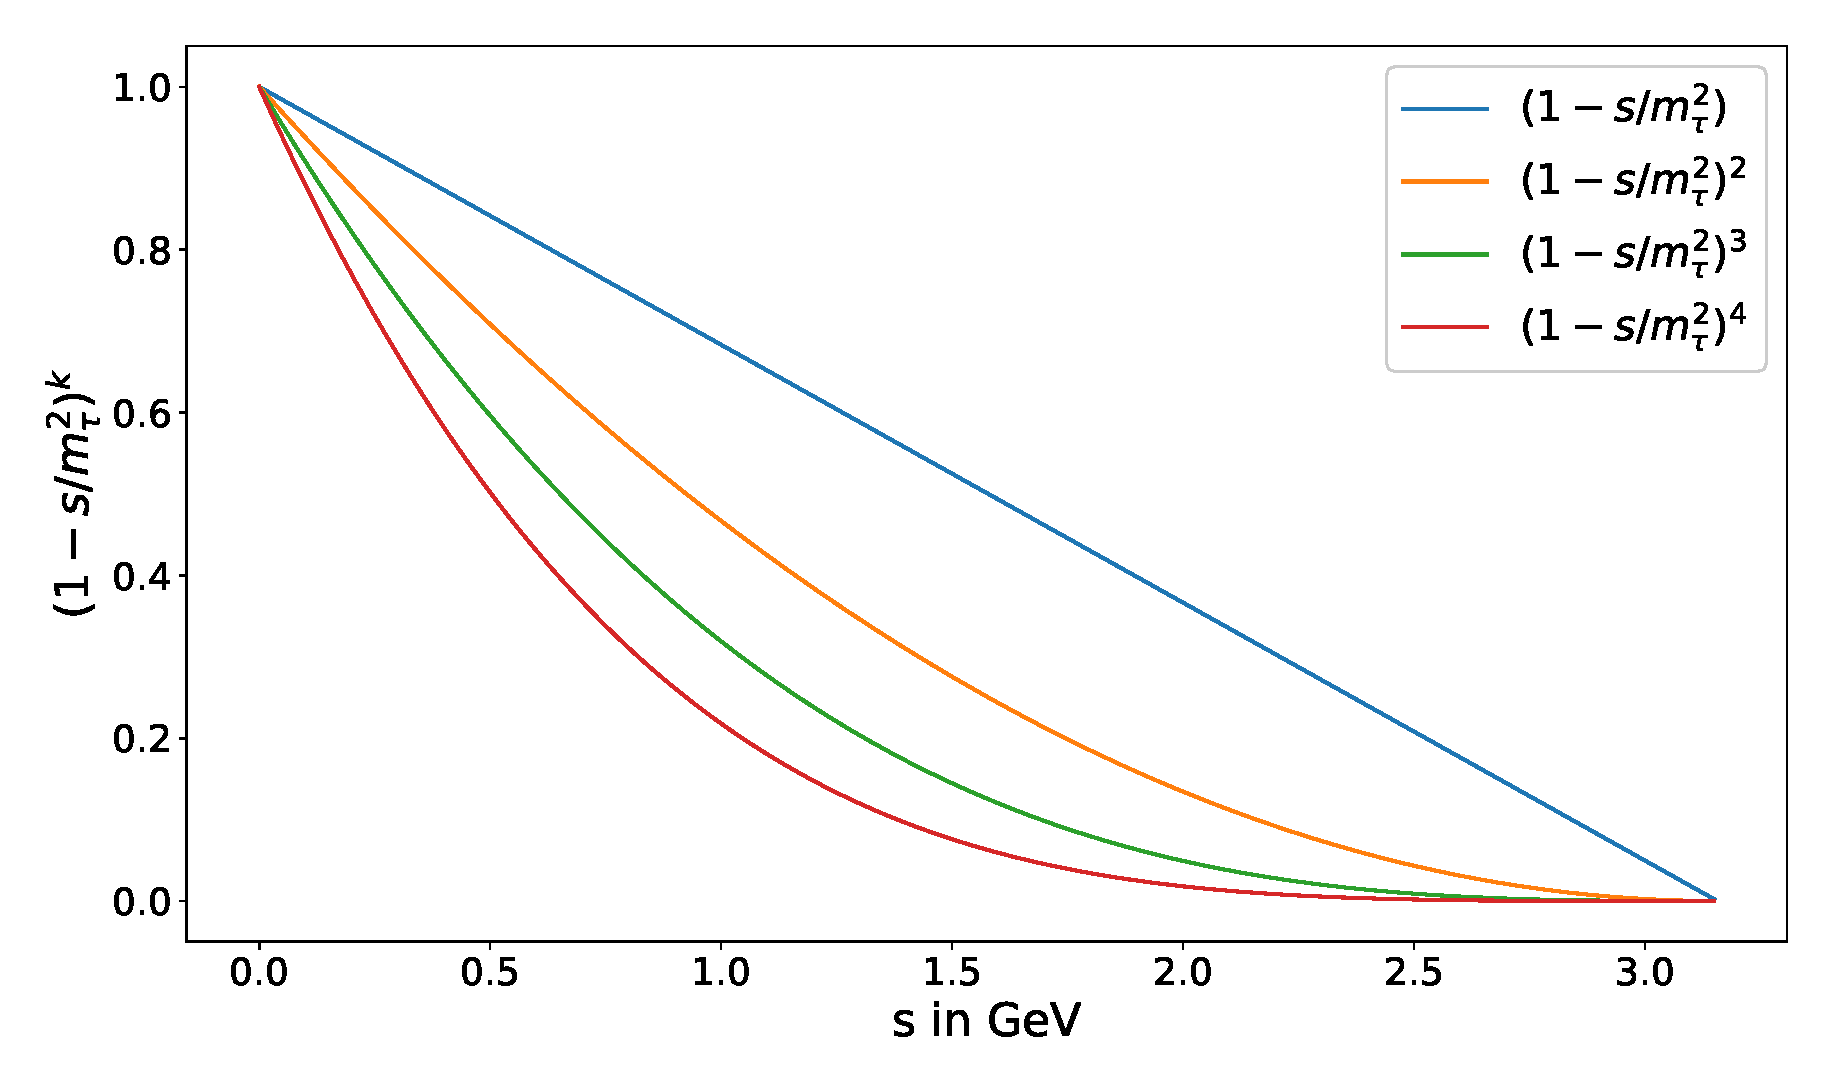
\includegraphics[width=\textwidth]{./images/monomialWeightGraphs.eps}
\end{frame}

\begin{frame}
  \frametitle{Weighting OPE Contributions}
  \begin{equation}
    \oint_{C} x^k \dif x = i \int_0^{2\pi}\left(e^{i \theta}\right)^{k+1} \dif \theta
    = \begin{cases} \mbox{\(2 \pi i\)} & \mbox{if } k=-1, \\ \mbox{0} & \mbox{otherwise} \end{cases}.
  \end{equation}
  \begin{equation}
    \left. R(x)\right\vert_{D=0,2,4,\dots} = \oint_{\abs{x}=1} \dif x \, x^{k-D/2} C^{(D)}
  \end{equation}
  active dimension
  \begin{equation}
    D = 2 (k+1)
  \end{equation}
  \begin{table}
    \centering
    \begin{tabular}{l|ccccccc}
      \toprule
      \textbf{monomial:} & \(x^0\) & \(x^1\) & \(x^2\) & \(x^3\) & \(x^5\) & \(x^6\) & \(x^7\)\\
      \textbf{dimension:} & \(D^{(2)}\) & \(D^{(4)}\) & \(D^{(6)}\) & \(D^{(8)}\) & \(D^{(10)}\) & \(D^{(12)}\) & \(D^{(14)}\)\\
      \bottomrule 
    \end{tabular}
    \caption{List of monomial and their corresponding ``active'' dimensions in the
      \textsc{ope}. Note that the perturbative contributions of the \textsc{ope}
      are always present.}
  \end{table}
\end{frame}



\section{Experiment}


\subsection{Inclusive Tau Decay Ratio}
\begin{frame}
  \frametitle{Inclusive Tau Decay Ratio}
  \begin{block}{Inclusive Tau Decay Ratio}
    \begin{ceqn}
      \begin{equation}
        R_{V/A,ud}(s_0) = 12 \pi \,\abs{V_{ud}}^2 S_{EW} \frac{1}{s_0} \int_0^{s_0} \dif s [ \omega^{(1+0)}(s) \rho_{V/A}^{(1+0)}(s) - \omega_L(s)\rho_{V/A}^{(0)}(s)]
      \end{equation}
    \end{ceqn}
  \end{block}

  \vfill

  \small
  \begin{equation}
    R_\tau = - \pi i \oint_{\abs{s}=m_\tau^2} \frac{\dif x}{x}(1-x)^3 \left[ 3(1+x)D^{(1+0)}(m_\tau^2x) + 4 D^{(0)}(m_\tau^2 x) \right]
  \end{equation}
  \hfill (\(x \equiv \frac{s}{m_\tau^2}\))
\end{frame}
\note[itemize]{
\item Spectral function can be determined via the inclusive tau decay ratio
\item We express the spectral function in therms of the Adler function 
}
\begin{frame}
  \frametitle{ALEPH data}
  \begin{columns}
    \begin{column}{0.5\textwidth}
      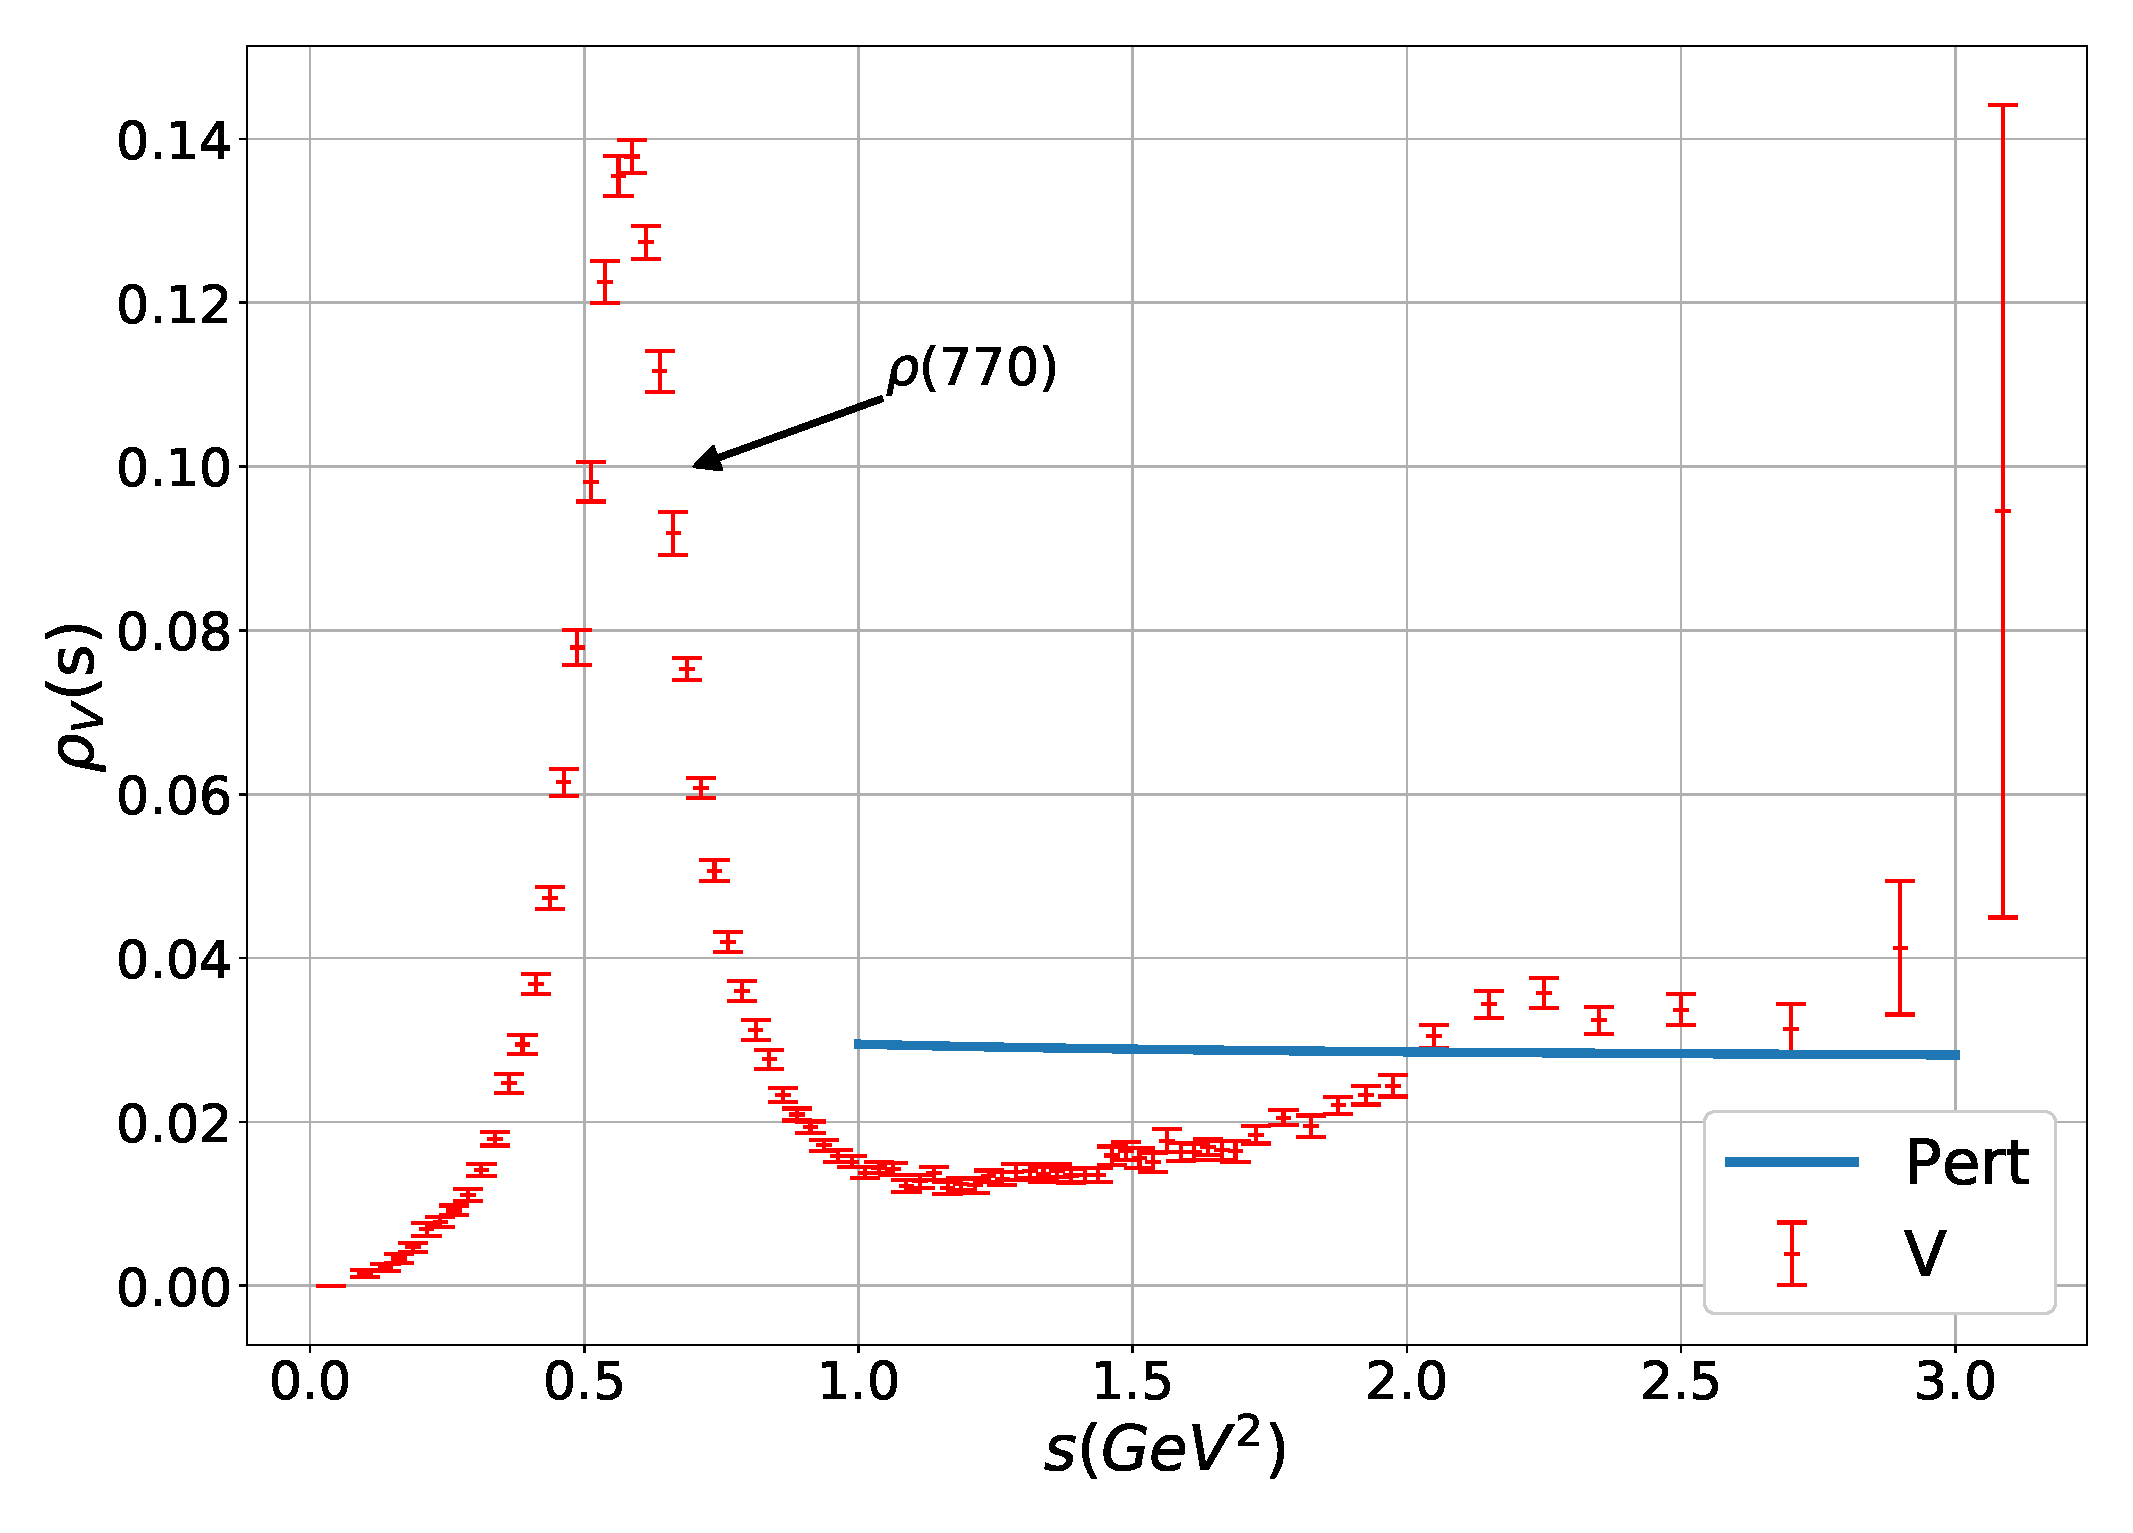
\includegraphics[width=\textwidth]{./images/specFuncAleph_V.eps}
    \end{column}
    \begin{column}{0.5\textwidth}
      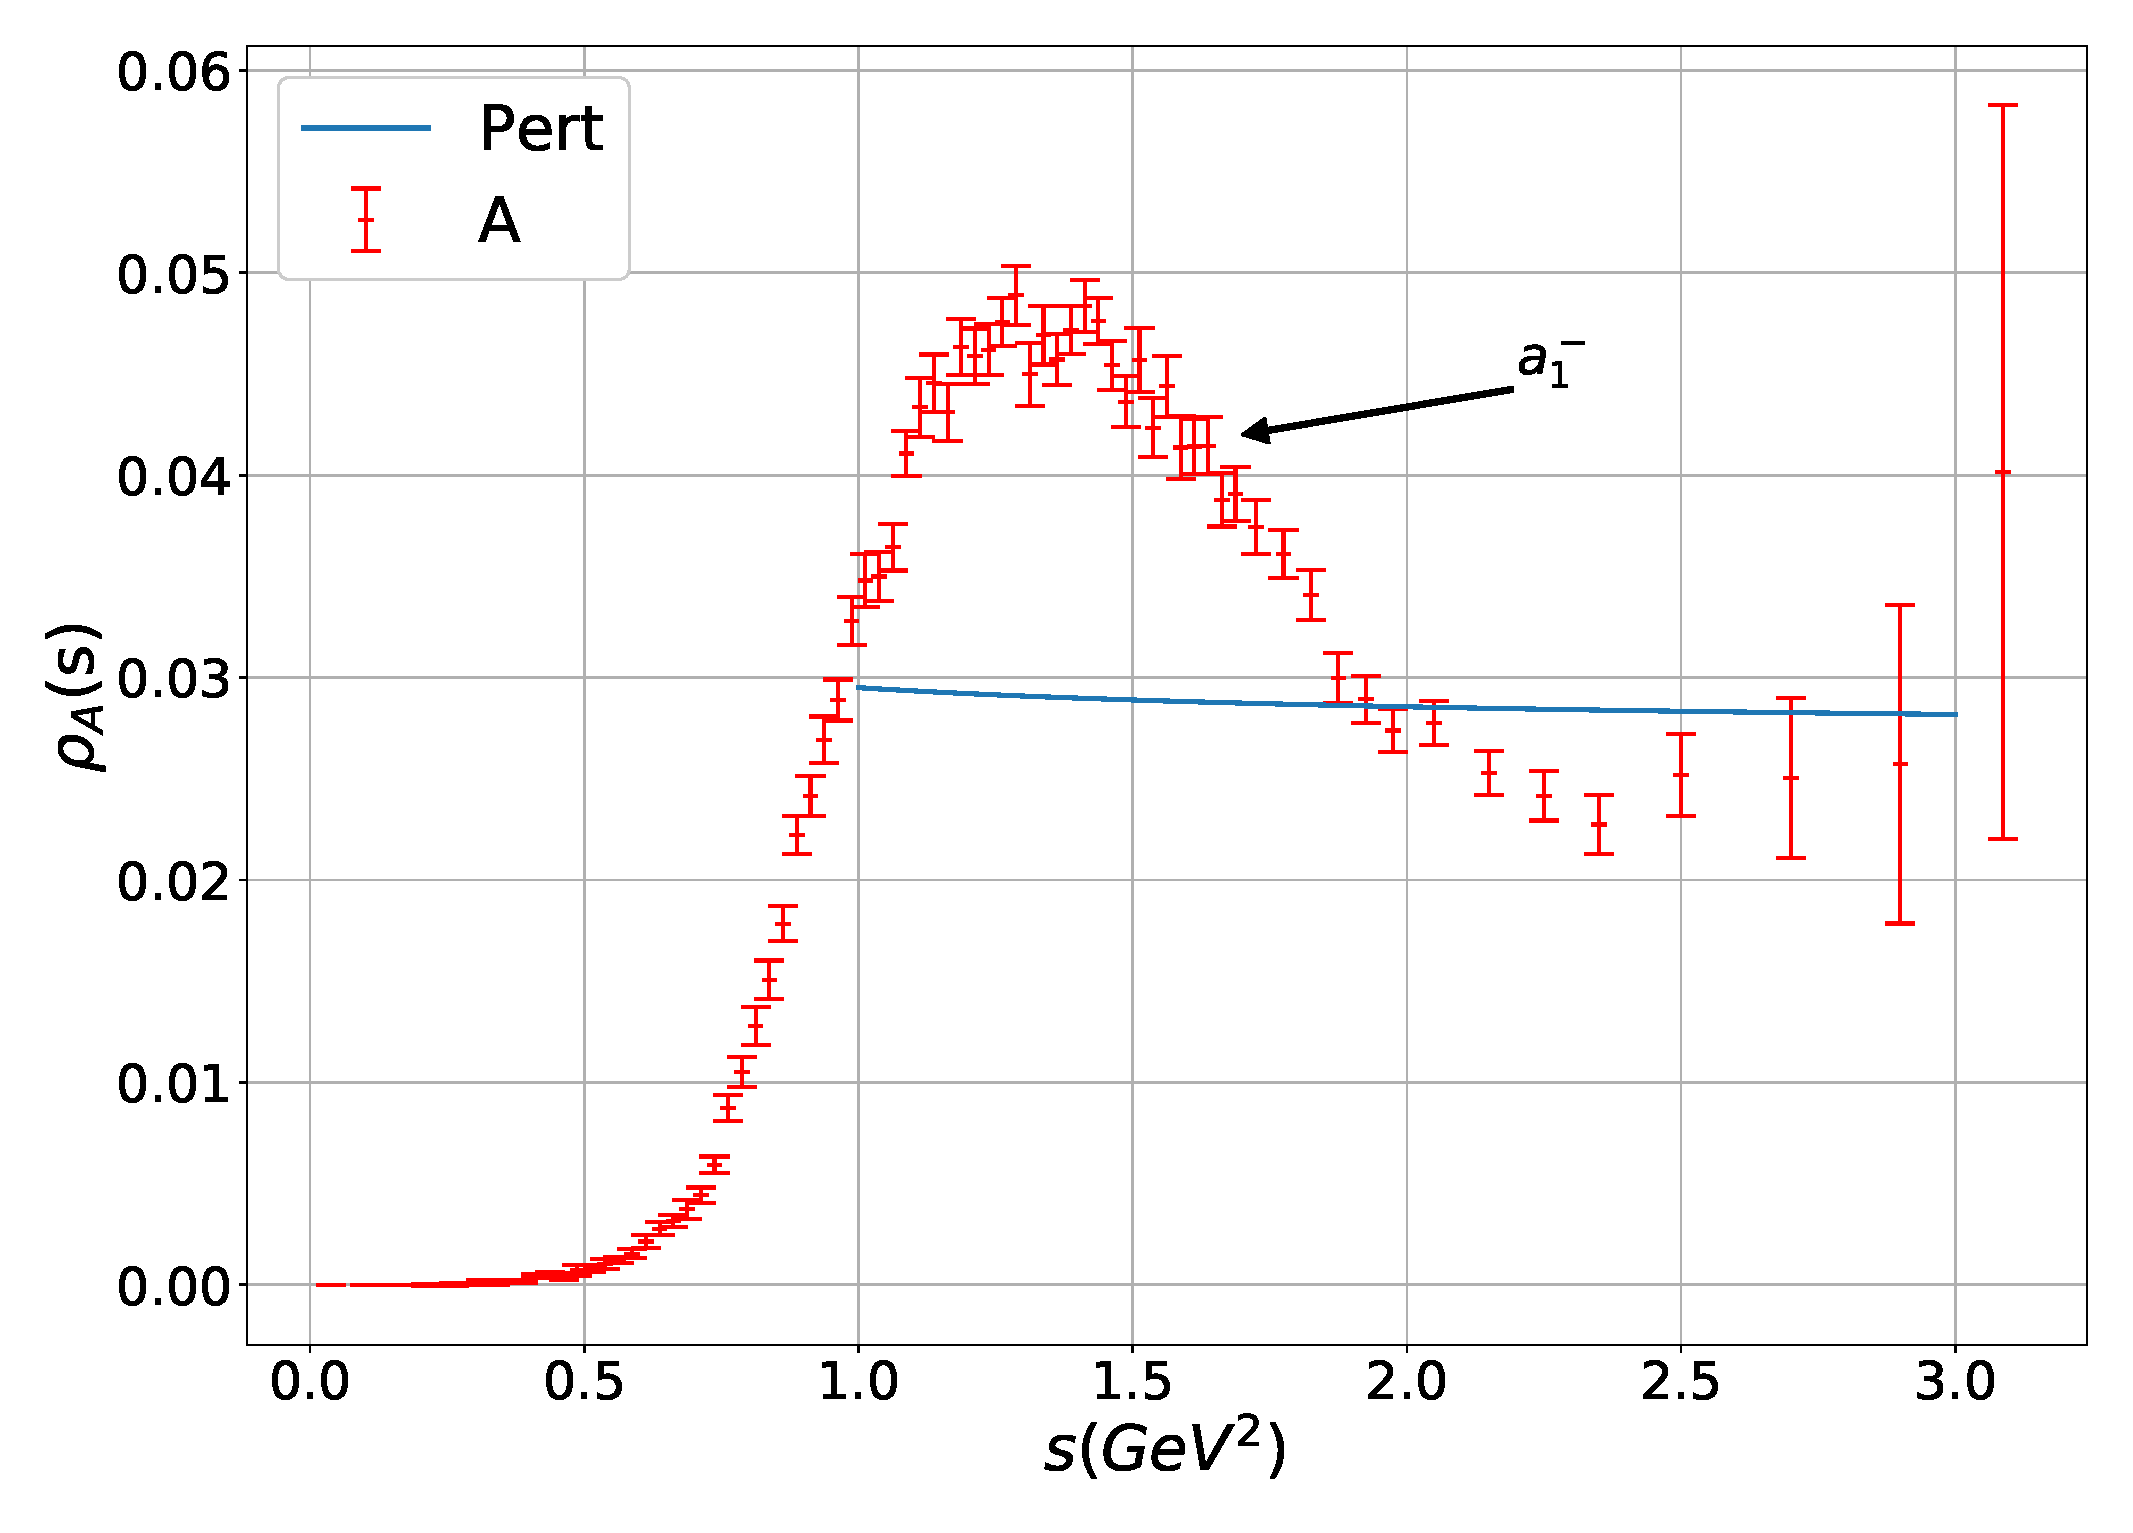
\includegraphics[width=\textwidth]{./images/specFuncAleph_A.eps}
    \end{column}
  \end{columns}
\end{frame}
\begin{frame}
  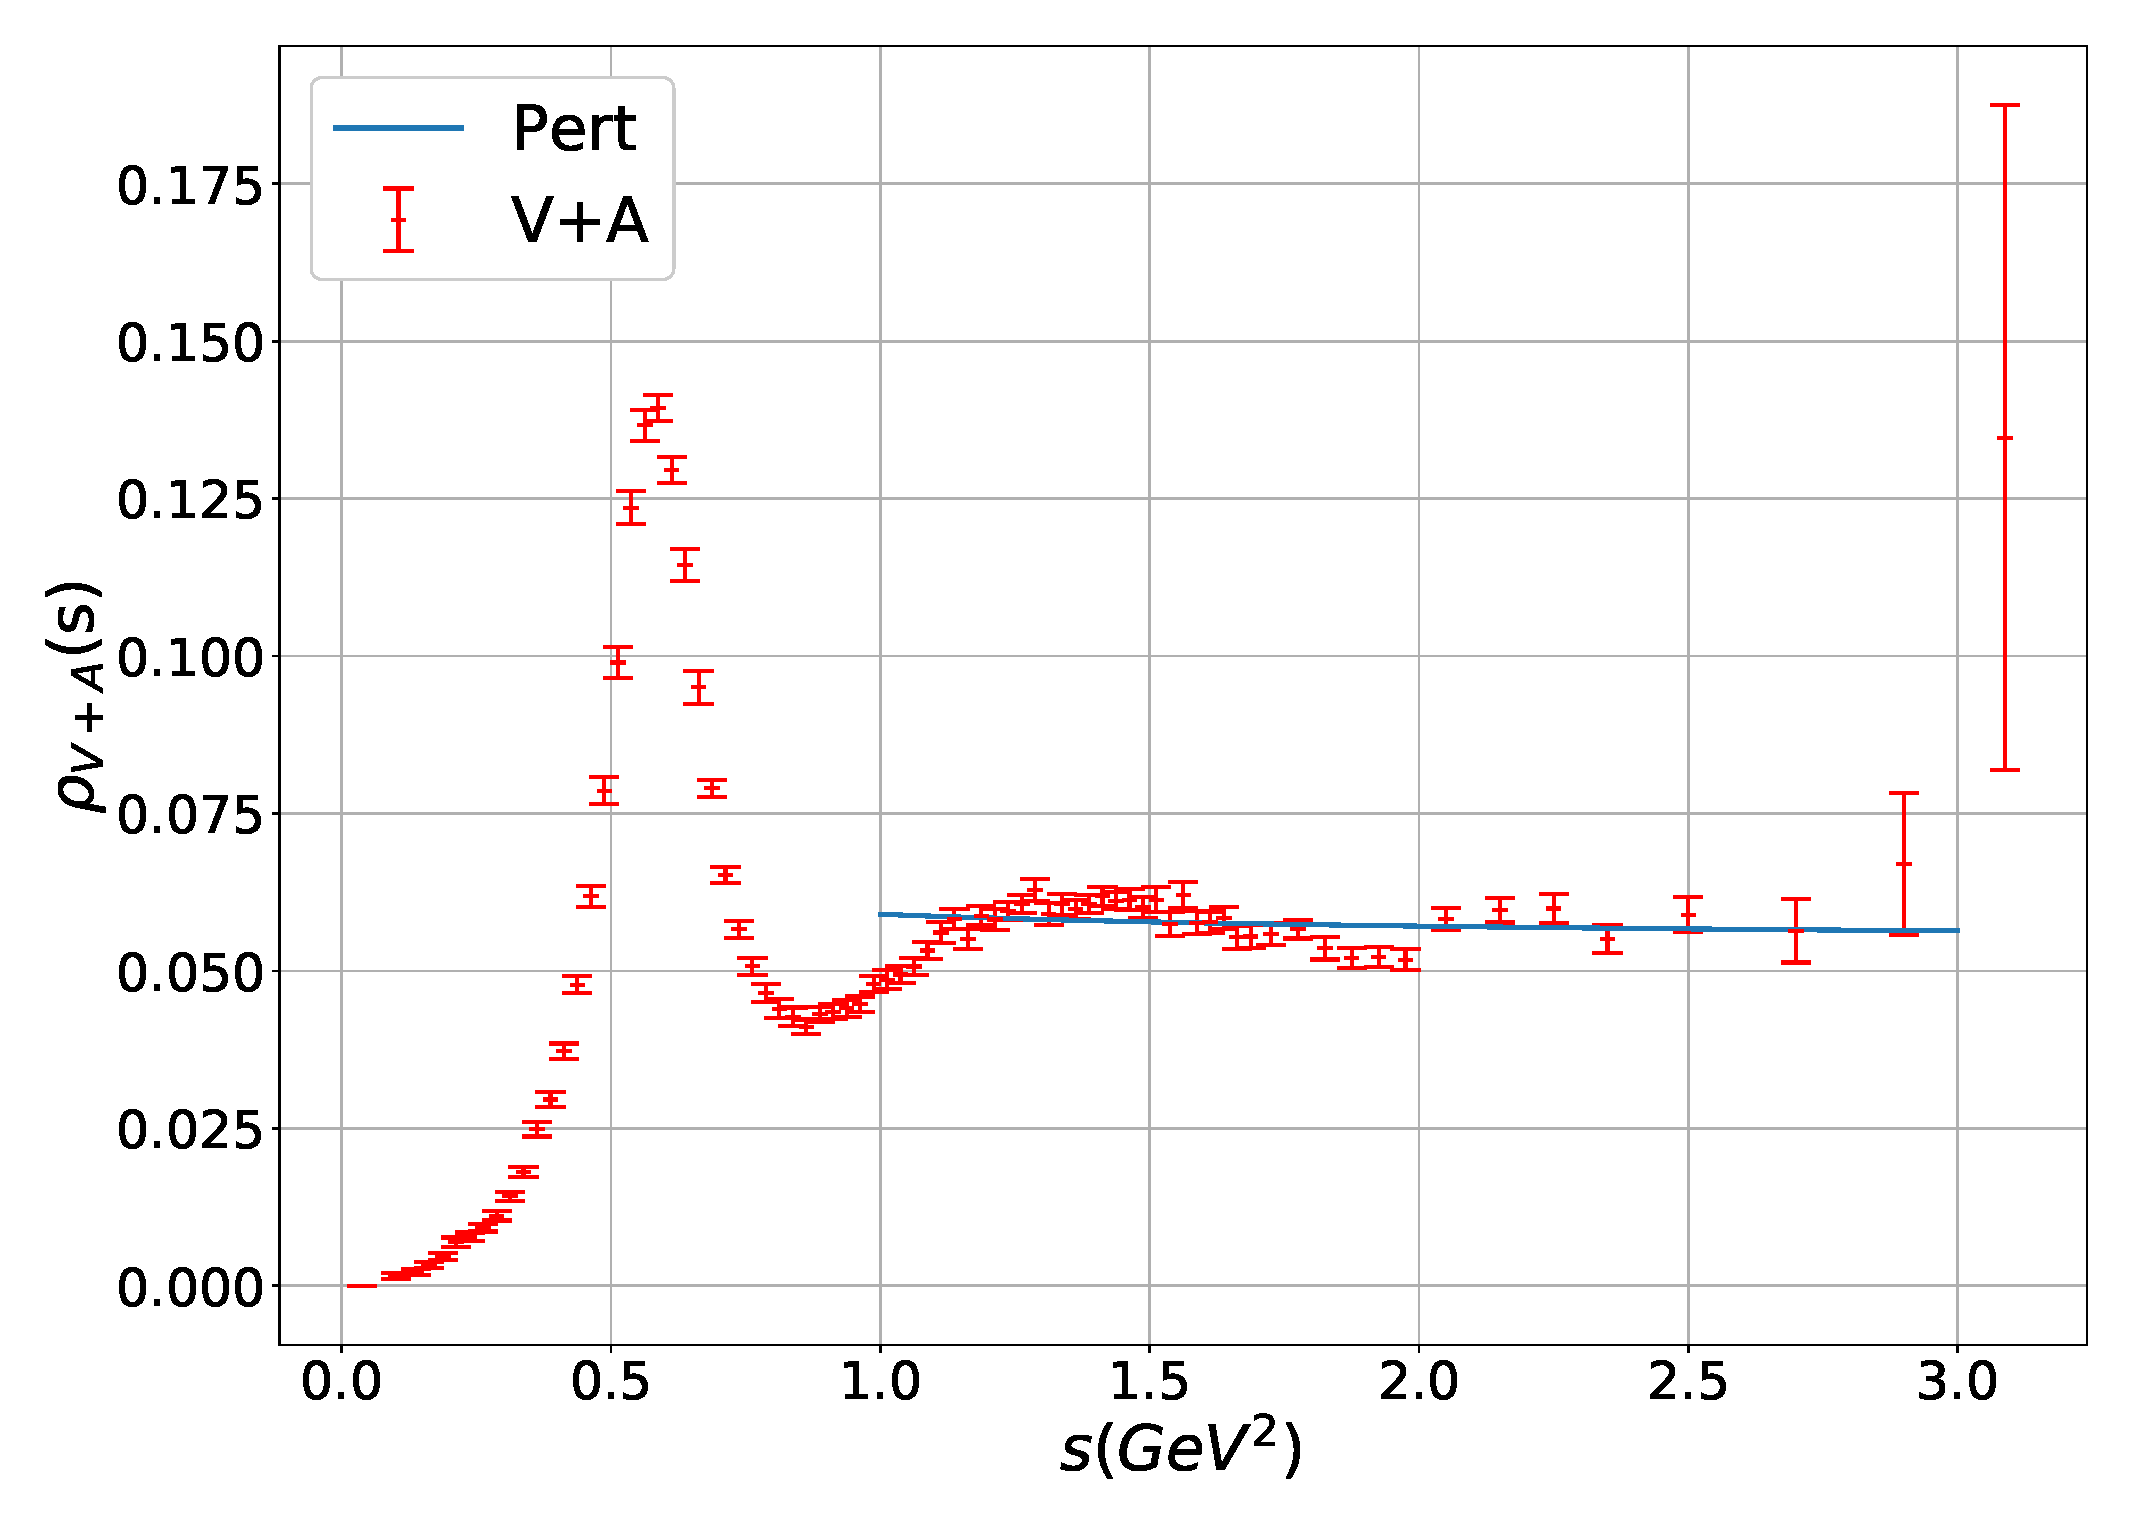
\includegraphics[width=\textwidth]{./images/specFuncAleph_VpA.eps}
\end{frame}
\begin{frame}
  \begin{equation}
    R_{\tau,V/A} = \frac{\mathcal{B}_{V/A}}{\mathcal{B}_e} = \int_0^{m_\tau^2} \dif s \frac{\sfm2_{V/A}(s)}{100 \mathcal{B}_e}
  \end{equation}
  \begin{equation}
    I_{exp,V/A}^\omega (s_0) = \frac{s_\tau}{100 \mathcal{B}_e s_0}
    \sum_{i=1}^{N(s_0)} \frac{\omega \left( \frac{s_i}{s_0} \right)}{\omega_\tau \left( \sfm2_{V/A}(s_i) \right)}
  \end{equation}
\end{frame}
\begin{frame}
  \begin{equation}
    \chi^2 = ( I_i^{exp} - I_i^{th}(\vec \alpha)) C_{ij}^{-1} (I_j^{exp} - I_j^{th}(\vec \alpha))
  \end{equation}
  \begin{equation}
    C_{ij} = \cov(I_i^{exp}, I_j^{exp})
  \end{equation}
  \begin{equation}
    \chi^2 \approx 1
  \end{equation}
\end{frame}

\section{Fits}
\subsection{Strategy}
\begin{frame}
  \frametitle{Parameters and Momenta}
  \begin{tabular}{ccc}
    \toprule
    \# (k, l) &\multicolumn{2}{c}{2 Moments} \\
    \midrule
    1 (1, 1)  & \(s_1\) & \(\omega_1\) \\
    2 (2, 1)  & \(s_2\) & \(\omega_1\) \\
    \bottomrule
  \end{tabular}
\end{frame}

\begin{frame}
  \resizebox{\textwidth}{!}{
    \begin{tabular}{ccccc}
      \toprule
      & Symbol & Term & Expansion & \textsc{ope} Contributions \\
      \midrule
      \parbox[t]{2mm}{\multirow{3}{*}{\rotatebox[origin=c]{90}{\small Pinched}}} & \(\omega_\tau\) & \((1-x)^2(1+2x)\) & \(1 - 3x^2 + 2x^3\) & \(D6, D8\) \\
      & \(\omega_{cube}\) & \((1-x)^3(1+3x)\) & \(1 - 6x^2 + 8x^3 - 3x^4\) & \(D6, D8, D10\) \\
      & \(\omega_{quartic}\) & \((1-x)^4(1+3x)\) & \(1 - 10x^2 + 20x^3 - 15x^4 + 4x^5\) & \(D6, D8, D10, D12\) \\
      \midrule
      \parbox[t]{2mm}{\multirow{3}{*}{\rotatebox[origin=c]{90}{\small Monomial}}} & \(\omega_{M2}\) & \(1 - x^2\) & \(1-x^2\) & \(D6\) \\
      & \(\omega_{M3}\) & \(1 - x^3\) & \(1 - x^3\) & \(D8\) \\
      & \(\omega_{M4}\) & \(1 - x^4\) & \(1 - x^4\) & \(D10\) \\
      \midrule
      \parbox[t]{2mm}{\multirow{4}{*}{\rotatebox[origin=c]{90}{\small Pinched \(+ x\)}}} & \(\omega_{1,0}\) & \((1 - x)\) & \(1 - x\) & \(D4\) \\
      & \(\omega_{2,0}\) & \((1 - x)^2\) & \(1 - 2x + x^2\) & \(D4, D6\) \\
      & \(\omega_{3,0}\) & \((1 - x)^3\) & \(1 - 3x + 3x^2 - x^3\) & \(D4, D6, D8\) \\
      & \(\omega_{4,0}\) & \((1 - x)^4\) & \(1 - 4x + 6x^2 - 4x^3 + x^4\) & \(D4, D6, D8, D10\) \\
      \bottomrule
    \end{tabular}
  }
\end{frame}

\subsection{Results}
\subsubsection{Pinched Weights without a Monomial term \(x\)}
\begin{frame}
  \frametitle{Kinematic Weight: \(\omega_\tau(x) \equiv (1-x)^2(1+2x)\)}
  \begin{tabular}{ccccccc}
    \toprule
    & \(s_{min}\) & \#\(s_0\)s & \(\alpha_s(m_\tau^2)\) & \(\rho^{(6)}\) & \(\rho^{(8)}\) & \(\chi^2/dof\)  \\
    \midrule
    \parbox[t]{2mm}{\multirow{1}{*}{\rotatebox[origin=c]{90}{\textsc{bs}}}}
    & 2.200 & 7 & 0.3274(42) & -0.82(21) & -1.08(40) & 0.21 \\
    \midrule
    \parbox[t]{2mm}{\multirow{5}{*}{\rotatebox[origin=c]{90}{\textsc{fopt}}}}
    % 1.500 & 23 & 0.3255(13) & -0.441(10) & -0.2909(34) & 2.00 \\
    % 1.525 & 22 & 0.3255(18) & -0.440(36) & -0.288(45) & 2.10 \\
    % 1.550 & 21 & 0.3265(16) & -0.478(36) & -0.343(50) & 1.81 \\
    % 1.575 & 20 & 0.3269(22) & -0.493(47) & -0.365(58) & 1.86 \\
    % 1.600 & 19 & 0.3272(23) & -0.506(51) & -0.384(64) & 1.94 \\
    % 1.625 & 18 & 0.3284(24) & -0.540(53) & -0.433(68) & 1.788 \\
    % 1.650 & 17 & 0.3283(24) & -0.550(57) & -0.448(74) & 1.90 \\
    % 1.675 & 16 & 0.3284(24) & -0.549(57) & -0.448(79) & 2.04 \\
    % 1.700 & 15 & 0.3281(24) & -0.538(63) & -0.430(87) & 2.19 \\
    % 1.750 & 14 & 0.3291(26) & -0.581(71) & -0.50(10) & 2.21 \\
    % 1.800 & 13 & 0.3293(27) & -0.589(77) & -0.51(11) & 2.43 \\
    % 1.850 & 12 & 0.3281(28) & -0.537(85) & -0.42(13) & 2.5 \\
    % 1.900 & 11 & 0.3272(29) & -0.493(93) & -0.35(15) & 2.65 \\
    % 1.950 & 10 & 0.3232(32) & -0.31(11) & -0.01(18) & 1.13 \\
    % 2.000 & 9 & 0.3234(34) & -0.32(12) & -0.03(21) & 1.31 \\
    & 2.100 & 8 & 0.3256(38) & -0.43(15) & -0.25(28) & 1.30 \\
    & \cellcolor{primary}2.200 & \cellcolor{primary}7 & \cellcolor{primary}0.3308(44) & \cellcolor{primary}-0.72(20) & \cellcolor{primary}-0.85(38) & \cellcolor{primary}0.19 \\
    & 2.300 & 6 & 0.3304(52) & -0.69(25) & -0.80(50) & 0.25 \\
    & 2.400 & 5 & 0.3339(70) & -0.91(39) & -1.29(83) & 0.10 \\
    & 2.600 & 4 & 0.3398(15) & -1.3(1.0) & -2.3(2.5) & 0.01  \\
    \bottomrule
  \end{tabular}
\end{frame}
\begin{frame}
  \frametitle{Cubic Weight: \(\omega_{cube}(x) \equiv (1-x)^3(1+3x)\)}
  \begin{tabular}{ccccccc}
    \toprule
    \(s_{min}\) & \#\(s_0\)s & \(\alpha_s(m_\tau^2)\) & \(\rho^{(6)}\) & \(\rho^{(8)}\) & \(\rho^{(10)}\) & \(\chi^2/dof\)  \\
    \midrule
    % 1.800 & 13 & 0.3305(37) & -0.493(76) & -0.48(12) & -0.66(20) & 2.99 \\
    % 1.850 & 12 & 0.3303(37) & -0.482(68) & -0.456(100) & -0.62(17) & 3.35 \\
    % 1.900 & 11 & 0.3249(29) & -0.280(20) & -0.088(21) & 0.088(55) & 1.58 \\
    % 1.950 & 10 & 0.3237(26) & -0.232(25) & 0.005(42) & 0.275(93) & 1.67 \\
    2.000 & 9 & 0.3228(26) & -0.196(27) & 0.075(28) & 0.420(56) & 1.96 \\
    \rowcolor{primary}
    2.100 & 8 & 0.3302(40) & -0.52(11) & -0.58(22) & -1.00(45) & 0.43 \\
    2.200 & 7 & 0.3312(43) & -0.56(12) & -0.68(23) & -1.23(50) & 0.55 \\
    2.300 & 6 & 0.336(11) & -0.78(47) & -1.17(98) & -2.38(22) & 0.29 \\
    2.400 & 5 & 0.3330(96) & -0.63(47) & -0.82(10) & -1.51(26) & 0.48 \\
    \bottomrule
  \end{tabular}
\end{frame}
\begin{frame}
  \frametitle{Quartic Weight:  \( \omega_{quartic}(x) \equiv (1-x)^4(1+4x)\)}
  \begin{equation}
    \begin{split}
      \alpha_s(m_\tau^2) = 0.3290(11), \quad \rho^{(6)}=-0.3030(46), \quad \rho^{(8)}=-0.1874(28), \\
      \rho^{(10)} = 0.3678(45) \quad \text{and} \quad \rho_{(12)}=-0.4071(77).
    \end{split}
  \end{equation}
\end{frame}

\subsubsection{Single Pinched Monomial Weights}
\begin{frame}
  \frametitle{\(\omega_{M2}(x) \equiv 1-x^2\)}
  \centering
  \begin{tabular}{ccccc}
    \toprule
    \(s_{min}\) & \#\(s_0\)s & \(\alpha_s(m_\tau^2)\) & \(\rho^{(6)}\) &  \(\chi^2/dof\)  \\
    \midrule
    2.100 & 8 & 0.3179(47) & -0.42(17) & 1.62 \\
    \rowcolor{primary}
    2.200 & 7 & 0.3248(52) & -0.77(22) & 0.38 \\
    2.300 & 6 & 0.3260(60) & -0.85(28) & 0.43 \\
    \bottomrule
  \end{tabular}
\end{frame}
\begin{frame}
  \frametitle{\(\omega_{M3}(x) \equiv 1-x^3\)}
  \centering
  \begin{tabular}{ccccc}
    \toprule
    \(s_{min}\) & \#\(s_0\)s & \(\alpha_s(m_\tau^2)\) & \(\rho^{(8)}\) &  \(\chi^2/dof\)  \\
    \midrule
    % 1.500 & 23 & 0.3160(28) & -0.523(65) & 2.4 \\
    % 1.525 & 22 & 0.3171(28) & -0.578(70) & 2.3 \\
    % 1.550 & 21 & 0.3173(29) & -0.587(76) & 2.42 \\
    % 1.575 & 20 & 0.3187(29) & -0.667(82) & 2.08 \\
    % 1.600 & 19 & 0.3189(30) & -0.679(87) & 2.19 \\
    % 1.625 & 18 & 0.3195(30) & -0.719(94) & 2.24 \\
    % 1.650 & 17 & 0.3205(30) & -0.783(99) & 2.1 \\
    % 1.675 & 16 & 0.3204(31) & -0.77(11) & 2.24 \\
    % 1.700 & 15 & 0.3206(31) & -0.79(11) & 2.39 \\
    % 1.750 & 14 & 0.3202(32) & -0.76(13) & 2.57 \\
    % 1.800 & 13 & 0.3217(33) & -0.88(14) & 2.41 \\
    % 1.850 & 12 & 0.3202(35) & -0.75(16) & 2.4 \\
    % 1.900 & 11 & 0.3202(36) & -0.75(18) & 2.67 \\
    % 1.950 & 10 & 0.3161(38) & -0.40(20) & 1.46 \\
    % 2.000 & 9 & 0.3148(39) & -0.28(22) & 1.47 \\
    2.100 & 8 & 0.3147(44) & -0.27(29) & 1.71 \\
    \rowcolor{primary}
    2.200 & 7  & 0.3214(49) & -1.01(39) & 0.41 \\
    2.300 & 6  & 0.3227(57) & -1.18(54) & 0.46 \\
    2.400 & 5  & 0.3257(67) & -1.58(74) & 0.39 \\
    2.600 & 4  & 0.325(10) & -1.54(1.53) & 0.58 \\
    2.800 & 3  & 0.326(21) & -1.69(4.03) & 1.17 \\
    \bottomrule
  \end{tabular}
\end{frame}
\begin{frame}
  \frametitle{Fourth Power Monomial: \(\omega_{M4}(x) \equiv 1-x^4\)}
  \centering
  \begin{tabular}{ccccc}
    \toprule
    \(s_{min}\) & \#\(s_0\)s & \(\alpha_s(m_\tau^2)\) & \(\rho^{(10)}\) & \(\chi^2/dof\)  \\
    \midrule
    % 1.500 & 23 & 0.3144(27) & -0.572(80) & 2.44 \\
    % 1.525 & 22 & 0.3155(27) & -0.655(90) & 2.34 \\
    % 1.550 & 21 & 0.3157(28) & -0.671(99) & 2.45 \\
    % 1.575 & 20 & 0.3171(28) & -0.80(11) & 2.1 \\
    % 1.600 & 19 & 0.3173(29) & -0.82(12) & 2.21 \\
    % 1.625 & 18 & 0.3180(29) & -0.88(13) & 2.24 \\
    % 1.650 & 17 & 0.3190(30) & -0.98(14) & 2.1 \\
    % 1.675 & 16 & 0.3189(30) & -0.97(15) & 2.24 \\
    % 1.700 & 15 & 0.3192(30) & -1.00(16) & 2.39 \\
    % 1.750 & 14 & 0.3188(32) & -0.96(19) & 2.58 \\
    % 1.800 & 13 & 0.3204(32) & -1.17(21) & 2.39 \\
    % 1.850 & 12 & 0.3190(34) & -0.95(26) & 2.4 \\
    % 1.900 & 11 & 0.3189(35) & -0.94(29) & 2.67 \\
    % 1.950 & 10 & 0.3149(37) & -0.31(34) & 1.47 \\
    % 2.000 & 9 & 0.3137(39) & -0.08(39) & 1.5 \\
    2.100 & 8  & 0.3136(43) & -0.07(54) & 1.75 \\
    \rowcolor{primary}
    2.200 & 7  & 0.3203(48) & -1.64(77) & 0.42 \\
    2.300 & 6  & 0.3216(56) & -2.01(1.13) & 0.47 \\
    2.400 & 5  & 0.3247(66) & -2.98(1.62) & 0.39 \\
    2.600 & 4  & 0.324(10) & -2.86(3.69) & 0.58 \\
    2.800 & 3  & 0.325(20) & -3.43(10.74) & 1.17 \\
    \bottomrule
  \end{tabular}
\end{frame}

\subsubsection{Pinched Weights with a Monomial Term \(x\)}
\begin{frame}
  \frametitle{\(\omega_{1,0} \equiv (1-x)\)}
  \centering
  \begin{tabular}{cccccc}
    \toprule
    & \(s_{min}\) & \#\(s_0\)s & \(\alpha_s(m_\tau^2)\) & \(\langle aGG \rangle_I\) & \(\chi^2/dof\)  \\
    \midrule
    \parbox[t]{2mm}{\multirow{3}{*}{\rotatebox[origin=c]{90}{\textsc{bs}}}}
    & 2.100 & 8 & 0.3176(47) & -0.0134(48) & 1.62 \\
    & \cellcolor{primary}2.200 & \cellcolor{primary}7 & \cellcolor{primary}0.3246(52) & \cellcolor{primary}-0.2262(59) & \cellcolor{primary}0.38 \\
    & 2.300 & 6 & 0.3260(60) & -0.2453(73) & 0.43 \\
    \midrule
    % 1.500 & 23 & 0.3369(26) & -0.0508(43) & 5.7 \\
    % 1.525 & 22 & 0.3376(24) & -0.0514(40) & 5.89 \\
    % 1.550 & 21 & 0.3395(28) & -0.0536(48) & 5.56 \\
    % 1.575 & 20 & 0.3395(28) & -0.0537(47) & 5.87 \\
    % 1.600 & 19 & 0.34047(68) & -0.05458(42) & 5.86 \\
    % 1.625 & 18 & 0.3414(30) & -0.0555(50) & 6.0 \\
    % 1.650 & 17 & 0.3418(30) & -0.0561(51) & 6.35 \\
    % 1.675 & 16 & 0.3430(32) & -0.0571(55) & 6.14 \\
    % 1.700 & 15 & 0.3436(33) & -0.0579(56) & 6.44 \\
    % 1.750 & 14 & 0.3457(36) & -0.0597(64) & 5.72 \\
    % 1.800 & 13 & 0.3462(37) & -0.0603(66) & 6.18 \\
    % 1.850 & 12 & 0.3479(43) & -0.0613(76) & 5.02 \\
    % 1.900 & 11 & 0.3489(46) & -0.0622(82) & 5.06 \\
    % 1.950 & 10 & 0.3528(65) & -0.067(12) & 1.69 \\
    % 2.000 & 9 & 0.3560(93) & -0.071(18) & 0.98 \\
    \parbox[t]{2mm}{\multirow{3}{*}{\rotatebox[origin=c]{90}{\textsc{fopt}}}}
    & 2.100 & 8  & 0.357(12) & -0.072(23) & 0.95 \\
    & 2.200 & 7 &  0.3593(97) & -0.079(19) & 0.2 \\
    & 2.300 & 6 & 0.3589(99) & -0.078(20) & 0.24 \\
    % 2.400 & 5 & 0.360(10) & -0.080(21) & 0.28 \\
    % 2.600 & 4 & 0.359(13) & -0.078(26) & 0.41 \\
    % 2.800 & 3 & 0.375(26) & -0.114(62) & 0.1 \\
    \bottomrule
  \end{tabular}
\end{frame}
\begin{frame}
  \frametitle{\(\omega_{2,0} \equiv (1-x)^2\)}
  \centering
  \begin{tabular}{ccccccc}
    \toprule
    & \(s_{min}\) & \#\(s_0\)s & \(\alpha_s(m_\tau^2)\) & \(\langle aGG \rangle_I\) & \(\rho^{(6)}\) & \(\chi^2/dof\)  \\
    \midrule
    % 1.500 & 23 & 0.3276(13) & -0.0077(10) & 0.330(35) & 2.62 \\
    % 1.525 & 22 & 0.3278(14) & -0.0078(10) & 0.330(38) & 2.75 \\
    % 1.550 & 21 & 0.3299(16) & -0.0092(12) & 0.333(37) & 2.31 \\
    % 1.575 & 20 & 0.3308(25) & -0.0098(13) & 0.334(47) & 2.32 \\
    % 1.600 & 19 & 0.3317(28) & -0.0105(14) & 0.335(54) & 2.38 \\

    % 1.650 & 17 & 0.3345(34) & -0.0124(17) & 0.342(62) & 2.15 \\
    % 1.675 & 16 & 0.3349(25) & -0.0127(15) & 0.342(51) & 2.28 \\
    % 1.700 & 15 & 0.3348(33) & -0.0126(18) & 0.342(58) & 2.47 \\
    % 1.750 & 14 & 0.3372(43) & -0.0145(23) & 0.341(71) & 2.34 \\
    % 1.800 & 13 & 0.3378(31) & -0.0149(20) & 0.339(58) & 2.54 \\
    % 1.850 & 12 & 0.3365(38) & -0.0138(25) & 0.346(60) & 2.72 \\
    % 1.900 & 11 & 0.3355(40) & -0.0128(28) & 0.354(59) & 2.97 \\
    % 1.950 & 10 & 0.3296(47) & -0.0073(34) & 0.418(58) & 1.57 \\
    % 2.000 & 9 & 0.3299(50) & -0.0076(39) & 0.414(64) & 1.83 \\
    % 2.100 & 8 & 0.3331(54) & -0.0108(45) & 0.361(76) & 1.9 \\

    \parbox[t]{2mm}{\multirow{3}{*}{\rotatebox[origin=c]{90}{\textsc{bs}}}}
    & 2.100 & 8 & 0.3207(48) & -0.0170(50) & -0.45(17) & 1.90 \\
    & \cellcolor{primary}2.200 & \cellcolor{primary}7 & \cellcolor{primary}0.3270(54) & \cellcolor{primary}-0.0254(61) & \cellcolor{primary}-0.77(21) & \cellcolor{primary}0.74 \\
    & 2.300 & 6 & 0.3253(63) & -0.0232(75) & -0.69(27) & 0.9  \\
    \midrule
    \parbox[t]{2mm}{\multirow{3}{*}{\rotatebox[origin=c]{90}{\textsc{fopt}}}} & 2.100 & 8 & 0.3331(54) & -0.0108(45) & 0.361(76) & 1.9 \\
    & 2.200 & 7  & 0.3401(57) & -0.0185(52) & 0.220(88) & 0.73 \\
    & 2.300 & 6  & 0.3383(68) & -0.0165(67) & 0.26(12) & 0.89 \\
    % & 2.400 & 5 & 0.3450(93) & -0.0243(99) & 0.10(17) & 0.71 \\
    % & 2.600 & 4 & 0.337(16) & -0.014(18) & 0.36(45) & 0.98 \\
    \bottomrule
  \end{tabular}
\end{frame}
\begin{frame}
  \frametitle{\(\omega_{3,0} \equiv (1-x)^3\)}
  \begin{adjustbox}{max width=\textwidth}
    \begin{tabular}{cccccccc}
      \toprule
      & \(s_{min}\) & \#\(s_0\)s & \(\alpha_s(m_\tau^2)\) & \(\langle aGG \rangle_I\) & \(\rho^{(6)}\) & \(\rho^{(8)}\) & \(\chi^2/dof\)  \\
      \midrule
      \parbox[t]{2mm}{\multirow{3}{*}{\rotatebox[origin=c]{90}{\textsc{bs}}}}
      & 2.000 & 9 & 0.3169(20) & -0.0123(34) & -0.29(12) & -0.05(24) & 2.0 \\
      & \cellcolor{primary}2.100 & \cellcolor{primary}8 & \cellcolor{primary}0.3239(40) & \cellcolor{primary}-0.0212(42) & \cellcolor{primary}-0.63(15) & \cellcolor{primary}-0.74(29) & \cellcolor{primary}0.46 \\
      & \cellcolor{primary}2.200 & \cellcolor{primary}7 & \cellcolor{primary}0.3251(17) & \cellcolor{primary}-0.02283(56) & \cellcolor{primary}-0.689(12) & \cellcolor{primary}-0.879(33) & \cellcolor{primary}0.56 \\
      \midrule
      \parbox[t]{2mm}{\multirow{3}{*}{\rotatebox[origin=c]{90}{\textsc{fopt}}}}
      % & 1.900 & 11 & 0.34281(92) & -0.01473(73) & -0.103(22) & -0.534(46) & 1.52
      % \\
      % & 1.950 & 10 & 0.34154(99) & -0.01304(61) & -0.050(17) & -0.389(44) & 1.42
      % \\
      & 2.000 & 9  & 0.33985(81) & -0.01124(43) & 0.002(10) & -0.242(26) & 1.59 \\
      & 2.100 & 8  & 0.3480(47) & -0.0201(36) & -0.264(89) & -1.03(28) & 0.31 \\
      & 2.200 & 7  & 0.3483(23) & -0.0204(41) & -0.27(15) & -1.05(40) & 0.41 \\
      % & 2.300 & 6 & 0.3522(64) & -0.0249(62) & -0.42(18) & -1.51(57) & 0.29 \\
      % & 2.400 & 5 & 0.3480(89) & -0.0199(100) & -0.25(33) & -0.96(10) & 0.39 \\
      \bottomrule
    \end{tabular}
  \end{adjustbox}
\end{frame}
\begin{frame}
  \frametitle{\(\omega_{4,0} \equiv (1-x)^4\)}
  \begin{adjustbox}{max width=\textwidth}
    \begin{tabular}{ccccccccc}
      \toprule
      & \(s_{min}\) & \#\(s_0\)s & \(\alpha_s(m_\tau^2)\) & \(aGGInv\) & \(\rho^{(6)}\) & \(\rho^{(8)}\) & \(\rho^{(10)}\) & \(\chi^2/dof\)  \\
      \midrule
      \parbox[t]{2mm}{\multirow{3}{*}{\rotatebox[origin=c]{90}{\textsc{bs}}}}
      & 1.950 & 10 & 0.31711(67) & -0.012432(24) & -0.30013(73) & -0.06785(16) & 0.26104(50) & 1.09 \\
      & \cellcolor{primary}2.000 & \cellcolor{primary}9 & \cellcolor{primary}0.3206(24) & \cellcolor{primary}-0.0167(14) & \cellcolor{primary}-0.455(38) & \cellcolor{primary}-0.373(67) & \cellcolor{primary}-0.36(14) & \cellcolor{primary}0.83 \\
      & \cellcolor{primary}2.100 & \cellcolor{primary}8 & \cellcolor{primary}0.3248(21) & \cellcolor{primary}-0.02230(47) & \cellcolor{primary}-0.6724(63) & \cellcolor{primary}-0.834(14) & \cellcolor{primary}-1.352(28) & \cellcolor{primary}0.23 \\
      \midrule
      \parbox[t]{2mm}{\multirow{2}{*}{\rotatebox[origin=c]{90}{\textsc{fopt}}}}
      & 1.950 & 10 & 0.3416(14) & -0.01306(83) & -0.050(22) & -0.390(59) & -0.50(19) & 1.71 \\
      & 2.100 & 8 & 0.3480(25) & -0.0201(27) & -0.264(91) & -1.02(23) & -339.00(20) & 0.41 \\
      \bottomrule
    \end{tabular}
  \end{adjustbox}
\end{frame}

\subsubsection{Comparison}
\begin{frame}
  \frametitle{Comparison}
  \centering \resizebox{\textwidth}{!}{
    \begin{tabular}{ccccccccc}
      \toprule
      & weight & \(s_{min}\) & \(\alpha_s(m_\tau^2)\) & \(\langle aGG \rangle_I\) & \(\rho^{(6)}\) & \(\rho^{(8)}\) & \(\rho^{(10)}\) & \(\chi^2/dof\)  \\
      \midrule
      \parbox[t]{2mm}{\multirow{4}{*}{\rotatebox[origin=c]{90}{\textsc{fopt}}}}
      & \(\omega_{\tau}\)    & 2.2 & 0.3308(44) & -            & -0.72(20) & -0.85(38) & - & 0.19 \\
      & \(\omega_{cube}\)    & 2.1 & 0.3302(40) & -            & -0.52(11) & -0.58(22) & -1.00(45) & 0.43 \\ 
      % & \(\omega_{quartic}\) & 2.0 & 0.3290(11) & - & -0.3030(46) &
      % -0.1874(28) & 0.3678(45) & 0.67 \\
      & \(\omega_{M2}\)     & 2.2 & 0.3248(52) & -            &  -0.77(22) & - & - & 0.38 \\
      & \(\omega_{M3}\)     & 2.2 & 0.3214(49) & -            & - & -1.01(39) & - & 0.41 \\
      % & \(\omega_{M4}\) & 2.2 & 0.3203(48) & - & - & - & -1.64(77) & 0.42 \\
      \midrule 
      \parbox[t]{2mm}{\multirow{3}{*}{\rotatebox[origin=c]{90}{\textsc{bs}}}}
      & \(\omega_{1,0}\)    & 2.2 & 0.3246(52) & -0.2262(59)  & -           & -          & -          & 0.38 \\
      & \(\omega_{2,0}\)    & 2.2 & 0.3270(54) & -0.0254(61)  & -0.77(21)   & -          & -          & 0.74 \\
      & \(\omega_{3,0}\)    & 2.1 & 0.3239(40) & -0.0212(42)  & -0.63(15)   & -0.74(29)  & -          & 0.46 \\
      % & \(\omega_X4}\) & 2.1 & 0.3248(21) & -0.02230(47) & -0.6724(63) &
      % -0.834(14) & -1.352(28) & 0.23 \\
      \bottomrule
    \end{tabular}
    }
\end{frame}


\section{Conclusions}
\begin{frame}
  \frametitle{Conclusions}
  \begin{columns}
    \begin{column}{.5\textwidth}
      \begin{itemize}
      \item \(\alpha_s(m_\tau^2) = 0.3261 \pm 0.0050\)
      \item \(\rho^{(6)} = -0.68 \pm 0.2\)
      \item \(\rho^{(8)} = -0.80 \pm 0.38\)
      \end{itemize}
    \end{column} \pause
    \begin{column}{.5\textwidth}
      \begin{itemize}
      \item DV not present if using single pinched weights in the V+A channel
      \item FOPT more valid than CIPT
      \item \(\alpha_s(m_Z^2) = 0.11940(60)\)
      \end{itemize}
    \end{column}
  \end{columns}
\end{frame}


\begin{frame}
  \centering
  \LARGE
  Questions
\end{frame}

\appendix
\begin{frame}
  Appendix
\end{frame}




\begin{frame}
  \printbibliography
\end{frame}

\end{document}
